%
% Settings file
%
%=======================================================================
%-------------This file controls various document settings--------------
%=======================================================================

%
% Should we compile for the Iliad (ebook reader), or regular A4
%
\newif\ifcompileiliad 
	\compileiliadfalse %Iliad (true) or regular A4 (false)?


%
% Set the fontsize and baselineskip here, use 13/15 for final document downscaling to 80% (UiB standard)
%
\newcommand{\TextSize}{13}
\newcommand{\BaseLineSkip}{15}
\newif\ifDownscaledFinalDoc
	\DownscaledFinalDoctrue		% Uib 13pt (true) or Regular 12pt (false)


%
% Compile draft (double line spacing)?
%
\newif\ifDraft
	\Draftfalse		% Draft (true) or Final (false)
	% Document settings file

%
% We use the book class
%
\ifcompileiliad
	\documentclass[10pt]{book}
\else
	\documentclass[12pt]{book}
\fi

%
% The geometry package allows consistent control of page layout
%
\ifcompileiliad
	\setlength{\parindent}{0pt}
	\setlength{\parskip}{3ex}
	\usepackage[papersize={122mm,160mm},
				hmargin=0.2cm,
				vmargin=0.2cm,
				tmargin=1.0cm,
				bmargin=0.4cm,
				dvips]
				{geometry}
\else
	\usepackage[paper = a4paper,         %To be shrunk to 80% when printed
				twoside,                 %Two-side mode, switches margins on 
				bindingoffset = 2mm,     %Offset for binding side of page
				hmargin = 25mm,          %Left and right margin
				vmargin = 25mm,          %Top and bottom margin
				dvipdfm]
				{geometry}
\fi	


% MY PACKAGES (MI)
\usepackage{subcaption}
\usepackage{tabularx,environ,amssymb}
\usepackage[ruled]{algorithm2e}

%
% Font settings
%
\usepackage[T1]{fontenc}	% Activate Type 1 fonts
\usepackage{mathptmx}       % Use Times font, also for math
\usepackage[scaled]{helvet} % for sans serif fonts (\textsf{...} or \sffamiliy)
\usepackage{sectsty}        % Change section and chapter header
\allsectionsfont{\usefont{OT1}{phv}{bc}{n}\selectfont} % Set chapter/section header to narrow helvectica (arial-like)
%\usepackage[scaled]{luximono} % for monospaced fonts (\texttt{...} or \ttfamily)

%
% Packages we need
%
\usepackage{graphicx}       % Handles figures
\usepackage[utf8]{inputenc} % We want æøå
\usepackage{amsmath}
\usepackage{amsfonts}
\usepackage[mathcal]{euscript} % For caligraphy fonts
\usepackage{booktabs}       % Publication quality tables
\usepackage{setspace}       % Easy setting of line spacing
\usepackage{forloop}		% For-loops!
\usepackage[numbers,
			sort&compress
			]{natbib}       % Sort numerical keys for multiple cites
\usepackage{hypernat}       % Avoid breaking 'backref' option of hyperref package
\usepackage{float}
\usepackage[dvipsnames]{color}   % named colors
\usepackage[procnames]{listings} % beautiful listings
\usepackage{units}				 % semantically represent numbers with units
\usepackage{tikz}	
\usepackage{subcaption}
     
\usepackage{amsthm}
%
% The hyperref package allows advanced hyperlinking functionality

\usepackage[dvipdfmx,        % Use dvipdf driver
			backref,         % List citing occurences in the References
			colorlinks,      % Colored links
			citecolor=blue,  % Color of cite links
			linkcolor=blue,  % Color of links
			urlcolor=blue,   % Color of urls
			]{hyperref}
%\newcommand{\aref}[1]{\autoref*{#1}} % Prevent links
\newcommand{\aref}[1]{\autoref{#1}} % Enable links


%
% Set fancy page header using fancyhdr package
% 
\usepackage{fancyhdr}
\pagestyle{fancy}

% Ensure that the chapter and section headings are in lowercase
\setlength{\headheight}{15pt}
\renewcommand{\chaptermark}[1]{\markboth{#1}{}}
\renewcommand{\sectionmark}[1]{\markright{\thesection\ #1}}

% Delete current section for header/footer
\fancyhf{}

% Define header/footer layout
\fancyhead[LE,RO]{\bfseries\thepage}
\fancyhead[LO]{\bfseries\rightmark}
\fancyhead[RE]{\bfseries\leftmark}
\renewcommand{\headrulewidth}{0.5pt}

% make space for the rule
\fancypagestyle{plain}{
	\fancyhead{} %get rid of the headers on plain pages
	\renewcommand{\headrulewidth}{0pt} % and the line
}

%
% Set header height to 30pt to make room for two rows in the header
% (useful if you have very long chapter names)
%
%\headheight 30pt


%
% Include user-defined macros
%
%====================================================
%-------------Macro definitions go here--------------
%====================================================

%
% Differentials
%
\newcommand{\tdiff}[2]{\ensuremath{\frac{d#2}{d{#1}}}}
\newcommand{\tdifforder}[3]{\ensuremath{\frac{d^{#2}#3}{d{#1}^{#2}}}}
\newcommand{\pdiff}[2]{\ensuremath{\frac{\partial#2 }{\partial#1}}}
\newcommand{\pdifforder}[3]{\ensuremath{\frac{\partial^{#2}#3}{\partial{#1}^{#2}}}}

%
% Linear algebra
%
\renewcommand{\vec}[1]{\ensuremath{\mathbf{#1}}}
\newcommand{\mat}[1]{\ensuremath{\mathbf{#1}}}
\newcommand{\tildemat}[1]{\ensuremath{\widetilde{\mat{#1}}}}


%
% Misc macros
%
\newcommand{\eref}[1]{~(\ref{#1})}
\renewcommand{\equiv}[0]{\ensuremath{:=}}
\newcommand{\etal}{\textit{et al. }}
\newcommand{\paperheader}[2]{\noindent\textbf{Paper #1}: \textit{#2}\\}
\newcommand{\paperitem}[3]{\noindent\textbf{Paper #1}: \textit{#2}\vspace{1em}\\\noindent #3\vspace{2em}}
\newcommand{\tfinal}{\ensuremath{T_{\text{f}}}}
\newcommand{\papernum}[1]{\textbf{#1}}


%
% Theorem environments
%
\newtheorem{definition}{Definition}


%
% Counters
%
\newcounter{ct}

%
% For loop to include papers
%
\newcommand{\includepaperpages}[2]
{
	\forloop{ct}{0}{\value{ct} < #2}
	{
		\begin{figure}[ht]
			\includegraphics[width=.99\textwidth]{#1\the\value{ct}.ps}
		\end{figure}
		\clearpage
	}
}


%
% TeX is very proud of its hyphenation engine, to the point where it 
% hyphenates _everything_ just to show off.  Increasing penalty for 
% hyphenation, and increase tolerance for underfull boxes can make 
% the text easier to read, at the expense of making the text less aligned
% to the right margin
%
\hyphenpenalty=10
\tolerance=1000


% Redefine include command -> input command
%\renewcommand{\include}{\input}

% Include only these chapters
%\includeonly{introduction}


%
% Set up the frontpage, with author, title, etc
%
\title{
{\fontsize{28}{30}\usefont{OT1}{phv}{bc}{n}\selectfont Optimization Problems in Communication Networks and Multi-Agent Path Finding}
	\author{
	\textbf{Marika Ivanova}\vspace{3cm}\\
		
\includegraphics[width=74mm]{figurer/uglo}\vspace{1em}\\
		Dissertation for the degree of Philosophiae Doctor (PhD)\vspace{3.5em}\\
		Department of Informatics\\
		University of Bergen
	}
	\date{Month year}
}

%====================================================
%------------------ BEGIN DOCUMENT ------------------
%====================================================
\begin{document}
%Cause all references in bibtex file to appear in the 'References' section, even
%if they are not explicitly cite'ed in the document
%\nocite{*}

%Set the fontsize and baselineskip, if something other than 10 or 12 is required
\ifDownscaledFinalDoc
	\fontsize{\TextSize}{\BaseLineSkip}
	\selectfont
\fi

%Double line spacing for draft
\ifDraft
	\doublespacing
\fi


%--------------------------------------------------------------------------------------------------
% FRONT MATTER
%--------------------------------------------------------------------------------------------------
\maketitle
\frontmatter
%\chapter{Scientific environment}

This is where you write the name of the subject/professional milieu involved in the study, faculty(faculties)/institute(s)/centre(s)/research groups/school of research.

Contractual joint venture partners should also be mentioned here. If these are represented by graphic symbols (logo etc.) the it should be on this page.

NB! Most organisations have guidelines concerning the use of their logo. These guidelines regulate who can use the logo, when the logo can be used and how. This is quite relevant when a logo is used together with information connected to other institutions/organisations. (A typical example would be rules concerning space between other written or graphic content.)

Remember to find out which guidelines apply and ensure that they are followed!
Most organisations will be able to provide a digital version of their logo in a suitable format.

\chapter{Acknowledgements}

I would like to thank\ldots

\chapter{Abstract}

%
This dissertation is a compilation of six research papers that are focused on three different topics summarized in the text.

The first three papers concern NP-hard problems arising in ad-hoc wireless communication discussed in Chapter 2.
In general, the task is to broadcast a message in a given network of wireless devices while minimizing the power consumption.
Problems in this category differ in requirements on the network connectivity, models of power consumption, and the ability of devices to initiate a signal transmission.
Some of the common features of these problems are that a device can simultaneously transmit a signal to all devices within its communication vicinity,
and that a signal can travel from its originator to its recipient via multiple intermediate devices.
The wireless networks are modeled by means of graph theory.
Solution techniques for these problems involve mainly methods of integer linear programming and inexact algorithms with or without performance guarantee.

The next paper is focused on the problem of minimum broadcast time.
Unlike the previous topic, devices in this problem are supposed to send a signal to up to one neighbouring device at a time.
The objective is to determine a sequence of signal transmission from a given set of source devices to the remaining ones while minimizing the time needed for spreading the signal.
Chapter 3 describes this problem in detail along with several related problems.
This problem is also studied from the integer linear programming as well as inexact algorithm perspective.
Continuous relaxations of the ILP models help to evaluate quality of the studied inexact methods.
The stronger model, the more accurate assessment it provides.

The last two papers are dedicated to problems belonging to path planning for multiple robots discussed in Chapter 4.
In general, these problems involve a group of agents (robots) initially deployed in an environment, and the task is to find a sequence of their moves
so that they reach pre-defined destination locations while optimizing a given criterion such as minimum makespan or minimum total arrival time.
The agents' movement must obey a set of given rules.
An extension of the problem considers agents divided into two (or more) adversarial teams, where the teams have either symmetric or asymmetric objectives.
After introducing the adversarial element, the problem of finding a winning strategy for a given team becomes PSPACE-hard, like many two player games with alternating turns.
%Additional requirement of preserving a communication possibility during the agets' movement has also been studied.

%The remainder of this chapter is structured as follows: 
%Section~\ref{sec:back} contains an overview of general underlying mathematical and algorithmical tools and methods employed in the attached papers.
%In Section~\ref{sec:smt}, we discuss ad-hoc wireless networks and describe several optimization problems in this area.
%In particular, we focus on the shared multicast tree problem and provide an insigt into its relation to other similar problems.
%Section~\ref{sec:mbt} introduces the minimum broadcast tree problem and discusses other relevant problems.
%In Section~\ref{sec:app}, we describe the problems in multi-robot path planning, and summarize their properties.
%An emphasis is given to the area protection problem.

%This is the introduction~\cite{deb01, pyprop}\ldots

%This is where you write the abstract, ref: 
%
%\vspace{1em}
%\noindent \textbf{Ӥ 6.6 Abstract of dissertation, press release}
%
%\vspace{1em}
%\noindent \textit{An abstract of the dissertation shall be prepared in English
%(1-3 pages), so that research environments in Norway and abroad may familiarize
%themselves with the results. The abstract shall accompany the dissertation.”}
%
%
%\vspace{1em}
%\noindent From  ”The Regulations for the degree philosophiae doctor (PhD) at the
%University of Bergen” 
%
%\vspace{1em}
%\noindent (There is an abstract template that has room for information about the debate,
%opponent etc that can be used as a handout.)

%\chapter{List of papers}

\begin{enumerate}

\item Author, \textit{Sometitle}, Somejournal \textbf{1}, 1, 1905.

\end{enumerate}

\tableofcontents
%\listoffigures
%\lstlistoflistings

%--------------------------------------------------------------------------------------------------
% MAIN MATTER
%--------------------------------------------------------------------------------------------------
\mainmatter

%
% Main chapters
%
\chapter{Background}\label{sec:back}

\section{Graph Terminology}\label{sec:back:graph}

A \emph{graph} $G$ is a pair $(V,E)$ of \emph{vertices} and \emph{edges}, where $E\subseteq {{V}\choose{2}}$.
If this inclusion is an equality, $G$ is said to be \emph{complete}.
 The set $A$ of arcs is derived from $E$ by considering both directions of orientation of the edges.
 Formally, $A=\left\{(i,j),(j,i):\left\{i,j\right\}\in E\right\}$.
A~\emph{path} in graph is a sequence of edges connecting a sequence of distinct vertices.
A~graph is said to be \emph{connected} if there exists a path between every two vertices, otherwise it is \emph{disconnected}.
A~\emph{cycle} of a graph $G$ is a subset of $E$ that form a path such that the first node of the path corresponds to the last. 
If $G$ contains a cycle, $G$ is called, \emph{cyclic}, otherwise it is called \emph{acyclic}.
\begin{definition}
A~tree is a graph that is connected and acyclic.
\end{definition}
For a vertex $v\in V$, a \emph{neighbourhood} of $v$ (open neighbourhood), denoted as $N(v)$, is the set of vertices adjacent to $v$.
The size of neighbourhood of $v$ is called a \emph{degree} of $v$.
A \emph{subgraph} of $G=(V,E)$ is a graph $G'=(V',E')$ such that $V'\subseteq V$ and $E'\subseteq E$.
This relation is often written as $G\subseteq G'$.
\begin{definition}
A spanning tree of graph $G=(V,E)$ is a tree $T=(V_T,E_T)$ such that $T\subseteq G$ and $V_T=V$.
\end{definition}

In a \emph{weighted graph} $G=(V,E,w)$, a \emph{weight} or \emph{cost} $w_e$ is associated witch each edge $e\in E$.
When use terms \emph{heavier, heavies} when comparing weights of different eges in a graph.
A~weight of $G$ is $\sum_{e\in E}w(e)$.
A~spanning tree of $G$ with minimum weight is called a \emph{minimum spanning tree} of $G$.
Similar concept is used in paths in graphs.
A~\emph{shortest path} from $u$ to $v$ in a weighted graph is a path consisting of edges of minimum sum of weights connecting $u$ and $v$.
\begin{definition}
	For a graph $G=(V,E)$ and a subset of vertices $D\subseteq V$, a Steiner tree of $G$ and $D$ is a tree $T=(V',E')$ such that $T\subseteq G$ and $D\subseteq V'$.
\end{definition}
Analogously in weighted graphs, a \emph{minimum Steiner tree} is a Steiner tree of minimum weight.

If edges have a direction associated with them, we call such a graph a \emph{directed graph}, and its edges are referred to as \emph{arcs}
Let $G=(V,A)$ be a directed graph. 
The downstream neighbourhood $N^-(v)$ of node $v$ is the set $\{(u,v): u\in V, (u,v) \in A\}$. 
Similarly, the upstream neighbourhood $N^+(v)$ is $\{(v,u): u\in V, (v,u) \in A\}$.
We use the standard notation $\text{deg}^-(v)=|N^-(v)|$ and $\text{deg}^+(v)=|N^+(v)|$.
These values are called \emph{in-degree} and \emph{out-degree} of $v$, respectively.
An~\emph{arborescence} rooted at vertex $r$ is a directed tree with arcs directed from $r$.
A~directed graph is \emph{strongly connected}, if for all pair of vertices $u,v\in V$, there is a path from $u$ to $v$ and from $v$ to $u$.

A graph is \emph{planar}, if it can be drawn in a plane without crossing edges.
According to this definition, every tree is planar. 
A graphical representation of a graph $G$ is determined by function $\Phi(G):V\mapsto\mathbb{R}\times\mathbb{R}$ that assigns a coordinate to each node in $V$. 
We say that $\Phi(G)$ is is an \emph{embedding of $G$ in a plane}.
\begin{definition}\label{def:planemb}
The embedding $\Phi(G)$ is planar if it is drawn in such a way that its straight line segments intersect only at their endpoints.
\end{definition}
Clearly, whenever $\phi(G)$ is planar, then also $G$ is planar. 
The opposite implication does not hold in general. 
If $\Phi(G)$ is not planar, any two edges that intersect each other are referred to as \emph{crossing}.

\section{Combinatorial Optimization}

Combinatorial optimization (CO) is a part of applied mathematics that tackles optimization problems over discrete structures.
It combines methods from graph theory, linear programming, combinatorics and the theory of algorithms.
In this section, we briefly introduce main concepts in CO used later in the text.
For a comprehensive rendition of this topic, an interested reader is referred to \cite{wolsey98} and \cite{nemhauser88}.

Combinatorial problems arise in many areas of computer science with a wide range of applications in various industrial disciplines 
such as production scheduling, logistics, communication network design and many more.
The core solving a problem by methods of CO is the identification of a discrete mathematical structure hidden in the problem,
and finding a sufficient abstraction.

CO concerns problems of minimization or maximization of an \emph{objective function} of several variables 
subject to inequality and equality \emph{constraints} and integrality restriction on at least some of the variables.
In this work, both the objective function and constraints are assumed to be linear.
Combinatorial problems are often formulated as \emph{mixed integer linear programs} (MILP) of the standard form
\begin{equation}
\begin{array}{r@{}l}
	\max\limits_{x,y}c^\top x + h^\top y & \\
	\text{subject to}& \\
	  Ax + Gy &\leq b, \\
	  x \in \mathbb{Z}^{n}_+, y & \in\mathbb{R}^{p}_+. 
\end{array}
\end{equation}

The problem instance is specified by the input data $c\in \mathbb{R}^n$, $h \in \mathbb{R}^n$, $A \in \mathbb{R}^{m\times n}$  $G \in\mathbb{R}^{m\times p}$ and $b \in \mathbb{R}^m$.
A MILP that is not in the standard form, for example if the objective is to minimize or if the constraints contain equalities, can be straightforwardly converted into the standard form.
If the integrality constraints are not present, we talk about a \emph{linear program} (LP)


The set of points $S=\{(x_0,y_0):  x_0 \in \mathbb{Z}^{n}_+, y_0  \in\mathbb{R}^{p}_+, Ax_0 + Gy_0 \leq b\}$ is called the \emph{feasible region},  
and a point $(x_0,y_0)\in S$ is referred to as a \emph{feasible point} (feasible solution) with \emph{objective function value} $c^\top x_0 + h^\top y_0$. 
A feasible point $(x^*,y^*)$ is called an \emph{optimal solution} if for every feasible points $(x_0,y_0)$ we have that $c^\top x_0 + h^\top y_0 \leq c^\top x^* + h^\top y^*$. 
Expression $c^\top x^* + h^\top y^*$ is then called the \emph{optimal value}. 

\subsection{Relaxation and Bounds}

\begin{definition}
	Let $S\subseteq \mathbb{R}^n$ and $\mathcal{F}$ be a MILP $\max\{f(x):x\in S\}$.
	The problem $\mathcal{R}: \max\{g(x):x\in T\}$ is a relaxation of $\mathcal{F}$ if and only if
	\begin{enumerate}
		\item $T\supseteq S$, and
		\item $g(x)\geq f(x) \text{ for all } x\in S$.
	\end{enumerate}
\end{definition}


Let $z^*$ and $\underline{z}$ be the optimal value of a MILP and its relaxation, respectively. 
Further, let $\bar{z}$ be the objective function value of some feasible point.
Then, $\underline{z}\leq z^* \leq \bar{z}$.
Values $\underline{z}$ and $\bar{z}$ are referred to as a lower bound and an upper bound, respectively.

A \emph{combinatorial relaxation} of a MILP is achieved by omitting one or more constraints. 
By omitting the integrality constraints of a MILP $\mathcal{F}$ we obtain its \emph{continuous relaxation}, also called \emph{LP relaxation}, denoted as LP$(\mathcal{F})$.

\subsection{Duality}

Consider a LP (\emph{primal})
\begin{equation}
	\max c^\top x   
	\text{ subject to } 
	  Ax \leq b, 
	  x   \geq 0. 
\label{eq:primal}
\end{equation}

We are looking for the best upper bound. 
If $x^*$ is an optimal solution to \eqref{eq:primal}, $y^\top Ax$ is a general linear combination of equations.
If it is possible to select a vector $y$ so that $y^\top Ax^*=c^\top x^*$, we have that $y^\top b \geq c^\top x^*$.
The best bound for any $x$ is than the optimal solution to the following LP (\emph{dual})
\begin{equation}
	\min b^\top y 
	\text{ subject to }
	  A^\top y \geq c,
	  y   \geq 0. 
\label{eq:dual}
\end{equation}
The relation between primal and dual LP is summarized by
\begin{proposition}
If the primal has an optimal solution $x^*$ then the dual has an optimal solution $y^*$ such that $c^\top x^* = b^\top y^*$.
\end{proposition}
For LPs duality provides a standard way to obtain upper bounds.
This concept can be applied to IPs.
\begin{definition}\cite{wolsey98}
The two problems
\begin{equation}
z=\max\{c(x): x\in X
\end{equation}
and
\begin{equation}
w=\max\{w(u): u\in U
\end{equation}
form a (weak)-dual pair if $c(x)\leq w(u)$ for all $x\in X$ and all $u\in U$. 
When $z=w$, they form a strong-dual pair.
\end{definition}
For obtaining an upper bound from LP relaxation it is necessary to solve the relaxed program to optimality, whereas any dual feasible solution provides an upper bound on $z$.
\begin{proposition}\cite{wolsey98}
The IP $z=\max\{cz: Ax\leq b, x\in Z^n_+\}$ and the LP $w^{LP}=\min\{ub:uA\geq c, u\in R^m_+\}$ form a weak dual pair.
\end{proposition}
\begin{proposition}\cite{wolsey98}
Suppose that the IP and D are a weak-dual pair.
\begin{enumerate}
\item If D is unbounded, IP is infeasible.
\item If $x^*\in X$ and $u^*\in U$ satisfy $c(x^*)=w(u^*)$, then $x^*$ is optimal for IP and $u^*$ is optimal for D.
\end{enumerate}
\end{proposition}

\subsection{Solution methods}

Linear programs are commonly solved in polynomial time by the \emph{simplex algorithm}.
A MILP can be solved by the \emph{branch and bound} (B\&B) method which may take exponential time.
These and other algorithms are an integral parts of most of the modern solvers such as CPLEX and GUROBI.

\section{Problems and Complexity}\label{sect:probcomp}

A \emph{computational problem} (problem) is an infinite collection of instances together with a solution for each instance.
A problem that can be posed as a yes-no question of the input values is referred to as \emph{decision problem}.
An example of a decision problem is the clique problem: Given a graph $G$ and an integer $k$, is there a clique in $G$ of size at least $k$?
In \emph{optimization problems}, the task is to find a ``best possible'' solution from among the set of all feasible solutions the problem instance.
The optimization version of the clique problem asks for finding the maximum clique in a given graph $G$.
An optimization problem can be solved by answering a sequence of decision problems:
Assume there is an oracle that is able to answer the clique problem for a given $(G,k)$.
The maximum clique problem can then be solved by answering its optimization version for $k=1,2,\dots$ until the answer is ``no'' for some $k'$, and so the maximum clique has the size $k'-1$.

Throughout this thesis, we use several well known concepts from the complexity theory, which we state in the following.
Detailed explanations of the terminology can be found in any textbook on this topic such as \cite{sipser06}.

An \emph{algorithm} is a procedure that solves a given problem in a finite number of steps.
Computational complexity of an algorithm is the amount of time needed for its run, and is measured in terms of the input size.
A \emph{polynomial} algorithm runs in time $\mathcal{O}(n^c)$, for some constant $c$ and input $w$ of size $|w|=n$.
A \emph{verifier} is an algorithm that determines whether a given certificate is a proof to the fact that $w$ is a yes-instance.
An example of a certificate in the clique problem is some subset of nodes of size $k$.
It can be verified in polynomial time whether there exists an edge between every two nodes.
\begin{definition}
	$P$ is the class of decision problems for which there exists a polynomial algorithm that solves them.
\end{definition}
\begin{definition}
	$NP$ is the class of decision problems for which there exists a polynomial verifier. 
\end{definition}
\begin{definition}
	Problem $X$ is polynomial time reducible to problem $X'$, if a polynomial computable function $f$ exists where for every $w$, 
	$w$ is a yes-instance of $X\Leftrightarrow f(w)$ is a yes instance of $X'$.
\end{definition}
\begin{definition}\label{def:npc}
	Decision problem $X$ is NP-complete if it satisfies:
	\begin{enumerate}
		\item $X$ is in NP.
		\item Every $X'$ in NP is polynomial time reducible to $X$.
	\end{enumerate}
\end{definition}
Remark:
A verifier does not decide whether a certificate is an optimal solution to a given optimization problem instance. 
When addressing optimization problems, we consider only the second property in Def.~\ref{def:npc}. 
If this property is satisfied, we say that the problem is NP-hard.

There are many well know examples of NP-hard problems, and they can be formulated as ILP.
Therefore, ILP itself is also NP-hard.

\begin{definition}
	PSPACE is the class of decision problems for which there exists an algorithm that solves them in a polynomial space.
\end{definition}
\begin{definition}\label{def:psc}
	Decision problem $X$ is PSPACE-complete if it satisfies:
	\begin{enumerate}
		\item $X$ is in PSPACE.
		\item Every $X'$ in PSPACE is polynomial time reducible to $X$.
	\end{enumerate}
\end{definition}
If $X$ satisfies only the second condition in Def.~\ref{def:psc} we say that $X$ is \emph{PSPACE-hard}.

\emph{Approximation algorithms} are polynomial algorithms that find approximate solution to NP-hard optimization problems with provable guarantee on the distance of the solution to the optimal one.
\begin{definition}\cite{williamson11}
A $\rho$-approximation algorithm for an optimization problem is a polynomial-time algorithm that for all instances of the problem produces a solution whose value is within a factor of
$\rho$ of the value of an optimal solution.
\end{definition}
The factor $\rho$ is called the \emph{approximation ratio} or \emph{performance guarantee}.
For minimization problems, $\rho > 1$, and for maximizations problems $\rho < 1$.
\begin{definition}
The class APX is the set of NP optimization problems that have an approximation algorithms with constant-ratio approximation algorithm.
\end{definition}
There are problems that are hard to approximate. 
A problem for which there is a constant $\rho$ such that it is NP-hard to find an approximation algorithm with approximation ratio better than $\rho$ is said to be APX-hard.
\begin{definition}\cite{williamson11}
A polynomial-time approximation scheme (PTAS) is a family of algorithms $\{\mathcal{A}_\epsilon\}$, where there is an algorithm for each $\epsilon > 0$ such that $\mathcal{A}_\epsilon$
is a $(1+\epsilon)$-approximation algorithm for minimization problems and $(1-\epsilon)$-approximation algorithm for maximization problems.
\end{definition}
\begin{proposition}
APX-hard problems do not admit PTAS.
\end{proposition}

\section{Path Planning}

Basic path-finding in (weighted) graphs is a well known task in computer science. The aim 
is to find a route between two selected vertices. We also use the term \emph{source} and
\emph{target} to refer to the initial vertex and target vertex, respectively.

%\subsubsection{Dijkstra's algorithm}

A shortest path can be found using \emph{Dijkstra's algorithm} \cite{dijkstra59}, which guarantees optimality.
Dijkstra’s Algorithm visits vertices in the graph starting with the source. 
It then repeatedly inspects the vertex which was not yet visited that lies closest to the source. 
It expands outwards from the source until it reaches the target. 
A drawback of this approach is that it may expand too many vertices that later turn out to lie very far from the target.

%\subsubsection{Best first search}

Another possibility is the greedy \emph{best first search} algorithm which can find the target faster, but the selected path is not guaranteed to be optimal.
Instead of expanding vertices close to the source, it selects those close to the target.
Obviously, which node is exactly the closest is not known without a previous preprocessing, and so it uses a heuristic estimation which guides the way towards the target.

%\subsubsection{A*}

The \emph{A*} algorithm combines the advantages of Dijkstra's and best first search algorithm.
It guarantees to find an optimal path and also exploits a heuristic estimation of the distance to the target which helps to avoid expanding unsuitable vertices.

The heuristic estimation is particularly useful when there is an incomplete information about the graph.
For that reason, A* is popular in video game development, where the exact distances can not be predicted due to a frequent change of the environment. 

Let us denote the source and target by $s$ and $t$, respectively.
The following values are considered for every vertex $v$:
\begin{itemize}
	\item $g_v$, a distance from $s$ to $v$,
	\item $h_v$, heuristic estimation of distance between $v$ and $t$, 
	\item $f_v=g_v+h_v$.
\end{itemize}
         % Introduction
\chapter{Power Minimizing Trees in Ad-hoc Wireless Networks}\label{sec:smt}

A Wireless Ad-hoc Network (WANET) is a decentralized type of wireless network.
Broadly speaking, there are two models of wireless networks: single-hop and multi-hop.
The single-hop model is based on the cellular network model that provides one-hop wireless connectivity between mobile hosts and static nodes known as base stations \cite{clementi01}.
This network type relies on a fixed backbone infrastructure that interconnects all base stations by wired links.
Unlike cellular and wired networks, WANETs depend on neither a wired infrastructure nor pre-determined interconnectivity.

The set of uniform wireless communication devices with fixed locations are connected via wireless links depending on 
distance between the nodes, their transmission power, error control scheme, background noise and interference.
Each device is equipped with an omnidirectional antenna with a communication range schematically illustrated in Fig. \ref{fig:omniantenna}.
Hence, a signal reaches all nodes within the communication range of its sender.
This range is determined by the power assigned to the sender, and this power can be adjusted over time.
The power necessary for relaying a signal to multiple devices is the maximum rather than the sum of the powers necessary to reach all intended receivers.
This feature is referred to as the \emph{wireless advantage} \cite{wieselthierXX}
Each device works as a transceiver, which means that it can both transmit and receive a signal.

\begin{figure}[htb!]
    \centering
    \begin{subfigure}[b]{0.35\textwidth}
        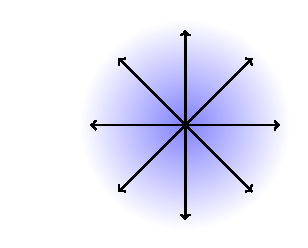
\includegraphics{figurer/omni-top.eps}
        \caption{Top view}
        \label{fig:omni-top}
    \end{subfigure}
    \begin{subfigure}[b]{0.55\textwidth}
        
\includegraphics{figurer/omni-side.eps}
        \caption{Side view}
        \label{fig:omni-side}
    \end{subfigure}
  \label{fig:omni}
  \caption{Omnidirectional antenna}
\end{figure}

The absence of infrastructure implies their quick deployment and simple configuration.
The recent years have witnessed an increasing interest in WANETs, motivated by numerous both civil and military applications and by the continual progression in wireless technologies.
Digital battlefield, disaster management, luggage handling in airports, context aware computing and mobile commerce are examples of the growing list of potential applications of WANETs \cite{younis06}.

Fig. \ref{fig:communication} depicts different types of communication in wireless networks.
Consider a group of devices and a specific sender who initiates a signal transmission. 
A \emph{unicast} means that there is a single recipient.
Whenever the recipients are all the remaining devices within the group, we talk about a \emph{broadcast}.
Finally, a \emph{multicast} means that only some of the devices must receive the message. 
The remaining ones do not have to, but they can serve as intermediate devices forwarding the signal.

The wireless devices are typically heavily energy constrained due to the use of batteries as their energy source.
Energy conservation in WANETs is therefore plentifully pursued research topic.
Most of the energy is spent on signal transmission \cite{halgamuge09}, 
and so it is desirable to design energy efficient transmission protocols that also satisfy certain requirements imposed on a WANET.

Various levels of connectivity are required on WANETs.
However, from a practical point of view, a topology which is ``too connected'' would often cause communication interference to occur even between nodes that are fart apart.
Theoretical as well as practical experimental results suggest that the communication graph in WANETs should be as sparse as possible while preserving connectivity \cite{blough02}.

Models considered for WANETs are usually deterministic, that is, they assume that the nodes are fully reliable. 
In reality, the nodes are devices that may be subject to temporary or permanent failure due to technical damage or battery draining.
This fact leads to considering \emph{probabilistic} models whose aim is to capture the real world more plausibly by taking into account the uncertain character of nodes' availability.
Besides minimizing the power consumptions of the network, it is also required to guarantee a certain level of reliability over the whole network.

\section{Wireless Sensor Networks}

A related paradigm to WANET are Wireless Sensor Networks (WSN) which attracted a wide range of disciplines where close interactions with the physical environment are essential.
WSNs consists of tiny sensor nodes, which act as both data generators and network relays \cite{akyildiz10}.
Each node act as a senosr, a microprocessor and a transceiver.
Sensor nodes have usually a fixed position and are powered by batteries.
Data measured  by sensors are transmitted via wireless communication links

There are countless of sensor types including seismic, electromagnetic and acoustic, suggesting a broad area of practical application areas such as 
military, environmental, health, home and industrial applications.

Multiple sensors are typically integrated into higher-level topologies varying in complexity.
These topologies can be divided into flat and hierarchical architecture \cite{mcgrath13}.
In a flat (peer to peer) architecture, every node has the same computational and communication capabilities.
In a hierarchical architecture, simple sensor nodes operate in close proximity to their respective cluster heads which possess more processing capacity than an ordinary sensor node.

WSNs are often built using the following configurations \cite{mcgrath13}:

\begin{itemize}
\item \emph{Point to point topology.} Links two endpoints either permanently or with the possibility of switching.
\item \emph{Bus topology.} Each node is connected to a shared communication bus, in which a signal is transmitted in both directions. 
\item \emph{Linear topology.} Two way link between one node and the next one, with two terminating nodes.
\item \emph{Ring topology.} A networks set up in a circular fashion is similar to linear topology, but does not contain the terminating nodes.
\item \emph{Star topology.} Consists of a single central node such as hub or a switch to which every node in the network is connected. 
An intelligent central node is required as all data traffic flows through it.
This topology is one of the most common WSN topologies.
\item \emph{Tree topology.} A hierarchy of nodes where in the highest level of the hierarchy is a single root node connected to one or many nodes in the level below.
The processing and power requirements in nodes increase as the data moves from the branches towards to root node.
\item \emph{Mesh topology.} Nodes disseminate their own data and also act as relays to propagate the data from other nodes.
The mesh topology can be partially connected  or fully connected (where there is a connection between every two nodes.
\end{itemize}

\section{Combinatorial optimization problems motivated by WANETs}

As indicated above, energy conservation is a crucial requirement in the design of WANETs. 
Combinatorial optimization is endowed with methods suitable for this task. 
It is necessary to introduce a formal network model in order to apply suitable mathematical tools.

\subsection{Network Model}

A WANET is modeled by a complete weighted graph $(G=(V,E),p)$, where the wireless devices are represented by nodes in $V$. 
As no power limit is imposed on the nodes, a transmission can be established between any two nodes, and thus $G$ is complete.
The function $p:E\to \mathbb{R}^+$ indicates the power requirement for sending a signal along a certain edge.
This requirement depends on distance and environmental properties, and is given by  $p_{ij}=d_{ij}^\alpha$, 
where $d_{ij}$ is the Euclidean distance between the devices represented by vertices $i$ and $j$, and $\alpha$ is the constant environmental factor typically valued between 2 and 4. 
Some sources state the relation $p_{ij}=\kappa d_{ij}^\alpha$, where $\kappa\geq$ is a transmission quality parameter.
The transmission range of a node $i$ depnends on the power supply $P_i$ assigned to it.
The overall power assignment to individual nodes induces a directed transmission graph (see example in Fig.~\ref{fig:transgraph}. 
On the other hand, for a given transmission graph, the power assignment to a node corresponds to the longest outgoing arc.
\begin{figure}[htb!]
  \centering
  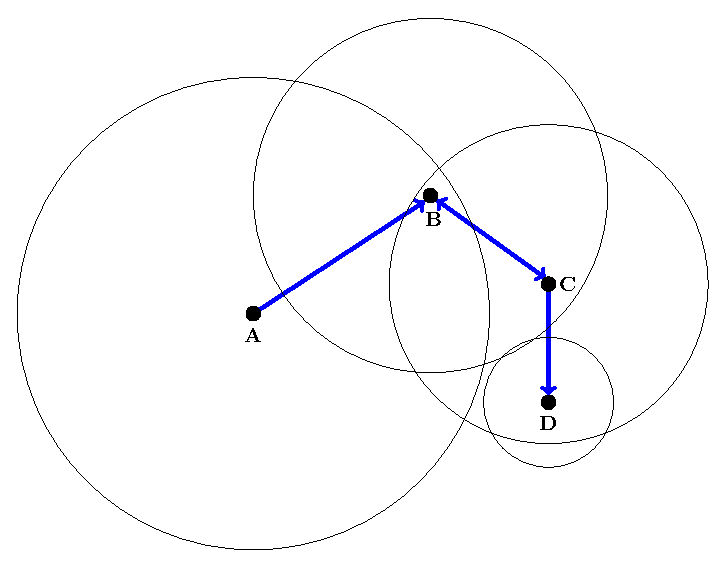
\includegraphics[scale=.8]{figurer/tran-graph.eps}
  \caption{Power assignment to nodes (circles)  and corresponding induced transmission graph (blue arrows)}
  \label{fig:transgraph}
\end{figure}
It is assumed that nodes are distributed in a Euclidean space, although it is also possible to consider more general variants..
In the following combinatorial problems motivated by WANETs, the task is to assign powers to individual nodes while satisfying certain criteria so that the overall power is minimized.
The total power is expressed by an objective function varying among the problem.

\subsection{Minimum Energy Broadcast}

The Minimum Energy Broadcast (MEB) problem consists of a set $V$ and a specified source $s\in V$, that is supposed to initiate a transmission.
All the remaining nodes must receive the signal via communication links induced by power assignment to the nodes.
\begin{problem}\label{prob:meb1}
Given a source $s\in V$, find a power vector $(P_1,P_2,\dots,P_n)\in\mathbb{R}^n$ of minimum sum s. t. 
there exists a path from $s$ to each $t\in V\setminus\{s\}$ in $G'=(V,E^P)$, where $E^P=\{(i,j)\in \vec{E}: p_{ij}\leq P_i\}$.
\end{problem}
An optimal solution differs for different transmission sources.
Hence, the nodes must by endowed with a mechanism that allows them to adjust their power level for a corresponding transmission session.
This places demands on the computational capacity and technological solution of the nodes.
The advantage of this concept lays in the optimality of each broadcast session.

The directed graph induced by power assignments as defined in Problem~\ref{prob:meb1} is not necessarily an arborescence.
However, MEB could be stated slightly differently:
\begin{problem}\label{prob:meb2}
Given a source $s\in V$, find an arborescence spanning $G$ rooted at $s$ such that 
the sum over weights of the heaviest outgoing arcs of all nodes is minimized.
\end{problem}

\begin{observation}
The objective function value of a given instance is equal in Problem~\ref{prob:meb1} and~\ref{prob:meb2}.
\end{observation}

MEB has received a significant attention during the last two decades.
The problem has been introduced in \cite{wieselthier00}, where the authors suggest three greedy heuristic methods:
MST algorithm, shortest path tree (SPT) algorithm and most notably the broadcast incremental power (BIP), which resembles Prim's algorithm for MST,
and improve them by a ``sweep'' operation removing unnecessary transmissions.
BIP gradually constructs a tree as follows:
\begin{itemize}
\item Initially, the tree $T$ contains only the source $s$, and all nodes have zero power assignment.
\item While there are some nodes outside of $T$
\begin{itemize}
	\item Find a node $v$ whose addition to $T$ results in a minimum increase of power assignments of some node $u$ already in $T$, and add $v$ to $T$.
	\item Increase  power assignment of $u$ so that $v$ is reached.
\end{itemize}
\item Sweep: Inspect non-leaf nodes in $T$ one by one, and if for some node $v$ there exists $u\in N^-(v)$ such that power assignment of $v$ is sufficient to reaches all nodes in $N^-(u)$, 
then the transmission of $u$ can eliminated.
\end{itemize}

In the MST algorithm, a MST is constructed, and subsequently the edges are oriented towards the leaves, starting from the source.
The last step is to assign power levels to each node according to the longest arc outgoing from that node.

The SPT algorithm establishes a minimum-cost path from the source node to every other node. The broadcast tree consists of superpositions of these unicast paths.

\subsubsection{Problem complexity and approximability}

NP-hardness results for both general and geometric MEB are provided in \cite{cagalj02} by reduction from \textsc{Set Cover} and \textsc{Planar 3-SAT}, respectively.
In the former case, the network topology is represented by a generic graph with arbitrary weights, whereas in the latter a Euclidean distance is considered.
The special case where $\alpha=1$, i.e., where the edge weights correspond to distances between the endpoints belongs to $P$.
An optimal solution is determined trivially by assigning minimum power sufficient to reach all nodes in a single hop, regardless of the nodes' arrangement.

The first analytical study of the three methods proposed in \cite{wieselthier00} is given in \cite{wan02}, where the authors provide quantitative characterization in terms of approximation ratios.
The MST algorithm is showed to have an approximation ratio between 6 and 12, while BIP between 13/3 and 12.
For the SPT algorithm the approximation ratio is at least $n/2$.
These results were gradualy improved in several works. 
The upper bound of the MST algorithm was improved to 6 in \cite{ambuhl05}, which closes the gap, and thus proves its optimality.
This upper bound is valid for BIP as well due to Lemma in \cite{wan02}:
\begin{lemma}
For any broadcasting among a point set $K$ in a 2-dimensional plane, the total energy required by the BIP algorithm is at most $\sum_{e\in \text{MST}(K)}d_e^\alpha$.
\end{lemma}
The lower bound was strengthened to 4.498 in \cite{bauer09}. 
This work also devises an implementation of BIP with improved time complexity $\mathcal{O}(|V|^2)$.

\subsubsection{Problem variants}

A special case, assuming that there are $k$ adjustable power levels $w_{i,1},w_{i,2},\dots w_{i,k}$ at each node $i$ is studied in \cite{liang02}.
This problem remains NP-hard which is proved by reducing \textsc{3-CNF-SAT} to it.
In addition, \cite{liang02} contains an approximation algorithm for this version of MEB with a performance guarantee $\mathcal{O}(n^\epsilon)$ and 
time complexity $\mathcal{O}((k+1)^{\frac{1}{\epsilon}} n^{\frac{3}{\epsilon}}$ for $\epsilon\in \left(0,1\right]$.
Further restriction pursued in \cite{liang02} assumes that each node has the same adjustable power levels, i.e., $w_{i,l}=w_{j,l}$ for $1\leq l\leq k$ and $1\leq i,j\leq n$.
In this scenario, another approximation algorithm which delivers a solution within $\mathcal{O}(\log^3 n)$ times the optimum is devised.

Probabilistic MEB where a node reliability is considered has also been investigated.
Three ILP formulations of probabilistic MEB together with suitable solving methods are developed in \cite{montemanni08}.
Another study of ILP formulations and suitable valid inequalities is pursued by \cite{barta10}.

A restriction of node locations can be imposed.
One example is a random grid network, where nodes are chosen independently and randomly from points of $\sqrt{n}\times\sqrt{n}$ square grid in the plane.
The probability distribution of existence of a node can be non-uniform.
A lower bound on the objective function is proved in \cite{calamoneri08} together with a near optimal construction method.
The 6-approximation of MST turns out to be too pessimistic for instances with restricted node locations which represent the real-life instances more closely.
Authors in \cite{flammini07} argue that the approximation ratio of MST algorithm can be considered close to 4 for practical instances.

\subsubsection{ILP models}

Integer linear programs for MEB are studied in various works.
Three ILP formulations are proposed in \cite{das03}.
The first formulation assumes exactly one transmission from the sourcde $s$, and at most one transmission from each node in $V\setminus\{s\}$.
This formulation operates with order of transmissions which helps to establish connectivity of the resulting solution.
Power asssignments are straightforwardly modeled by continuous variables for each node leading to an objective function minimizing their sum.

The same objective function is used in the second formulation.
On the contrary, the second formulation allows at least one transmission from the source and arbitrary number of transmission from the other nodes.
The necessary subtour elimination is achieved by additional ``sequencing variables'' proposed for the \textsc{Travelling Salesman Problem}.

The last formulation is built upon a single-commodity network flow model and its interpretation follows from the second formulation.

A similar formulation is proposed in \cite{yuan05}, where the continuous power variables for each node are replaced by binary variables $y_{ij}=1\Leftrightarrow$ the power of node $i$ equals $p_{ij}$,
and the connectivity is achieved by multi-commodity flow variables.

Authors in \cite{haugland11} provide a formal proofs that using binary power variables instead of continuous ones leads to a stronger formulation,
which can be further strengthened by introducing the multi-commodity flow variables.

\subsubsection{Planarity of an optimal solution}

Alternatively, a MEB instance can be defined by $G=(V,E)$ and its embedding $\Phi(G)$ in a plane.
We recall from Section \ref{sect:back:graph} that an embedding of a graph in a plane assigns coordinates to nodes in a Euclidean plane.
These coordinates implicitly imply distance $d_{ij}$ between every two nodes $i$ and $j$.

We address the question whether an optimal solution to various MEB instances have planar embedding.
To the best of our knowledge, the available literature does not provide results on this topic.
The unpublished findings presented below assume the MEB problem as stated by Def.~\ref{def:meb:tree}.

By inspecting a large number of instances and their optimal solution, the planarity of the optimum cannot be guaranteed in general, even though in majority of cases, the optimum is indeed planar.
\begin{proposition}\label{prop:mebplan}
Consider nodes 4 nodes in an instance of MEB that form a convex quadrilateral $ABCD$.
If two non-adjacent sides of the quadrilateral are shorter than the shorter diagonal, then in an optimal solution, edges with endpoints in $ABCD$ do not cross each other.
\end{proposition}
\begin{proof}
Consider the quadrilateral as depicted in Fig~\ref{fig:quad}. 
\begin{figure}[htb!]
  \centering
  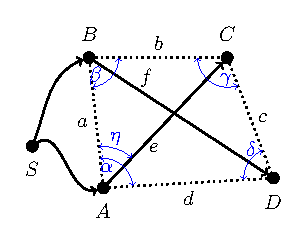
\includegraphics[scale=1.4]{figurer/quadrilat.eps}
  \caption{Four nodes forming a convex quadrilateral}
  \label{fig:quad}
\end{figure}
Without loss of generality, let $d_{AC}\leq d_{BD}$, $d_{AB}\leq d_{AC}\leq d_{BC}$ and $d_{CD}\leq d_{AC}\leq d_{AD}$.
By the law of cosine, we have that 
$$
\cos{\beta}=\frac{d^2_{AB} + d^2_{BC} - d^2_{AC}}{2d_{AB}d_{BC}} \text{~~~ and ~~~}\cos{\delta}=\frac{d^2_{CD} + d^2_{AD} - d^2_{AC}}{2d_{CD}d_{AD}}.
$$
Since both numerators are positive, both $\beta$ and $\delta$ are acute, which immediately implies that $\alpha $ and $\gamma$ are obtuse.

Let $T=(V,A_T)$ be an optimal solution to the given instance.
If $(AC)\in A_T$ and $(BD)\in A_T$, $(A,C)$ covers $B$ due to the wireless advantage, and $(B,D)$ covers $C$ because $\gamma$ is obtuse.
Then, by replacing $(AC)$ with $(AB)$ we get rid of the crossing and all four nodes are covered.
If $(AC)\in A_T$ and $(DB)\in A_T$, $(DB)$ covers both $A$ and $C$ as $\alpha$ and $\gamma$ are obtuse, thus $(A,C)$ can be removed without disconnecting the solution.
The remaining cases are symmetric.
\end{proof}
If the condition that the shorter sides must not be adjacent is not met in Prop.~\ref{prop:mebplan}, a crossing may occur, as example in Fig.~\ref{fig:mebnonplan} demonstrates.
\begin{figure}[htb!]
  \centering
  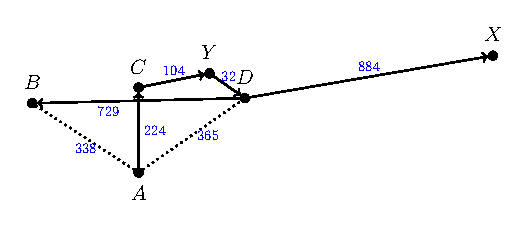
\includegraphics[scale=1.4]{figurer/mebnonplanar.eps}
  \caption{A unique optimal solution with crossing to a Euclidean instance of  MEB with source in node $A$.
  The blue edge weights correspond to the power requirements between two nodes. 
  The nodes have coordinates $A=[75,63]$, $B=[50,77]$, $C=[49,63]$, $D=[50,50]$, $X=[45,22]$ and $Y=[47,55]$.
  For convenience, lengths of edges in the figure are not proportional.}
  \label{fig:mebnonplan}
\end{figure}

\subsection{Range Assignment Problem}

In the range assignment problem (RAP) the task is to minimize the total power consumed under the constraint 
that adequate power is provided to the nodes to ensure a strong connectivity of the graph.
Formally, the problem is stated as follows:
%Therefore, only one broadcast tree is stored which is common for all possible sources.
\begin{problem}
Find a power vector $(P_1,P_2,\dots,P_n)\in\mathbb{R}^n$ of minimum sum such that the induced graph $G'=(V,E^P)$ is strongly connected, 
where $E^P=\{(i,j)\in \vec{E}: p_{ij}\leq P_i\}$.
%every where $E^P=\{(i,j)\in E: p_{ij}\leq P_i\wedge p_{ij}\leq P_j\}$.
\end{problem}
In \cite{kirousis00}, it is shown that for instances consisting of collinear points, there exists an algorithm that solves the problem to optimality in $\mathcal{O}(n^4)$.
The authors further prove by reduction from \textsc{Vertex Cover} that RAP in 3-dimensional Euclidean space is NP-hard,
and that there exists a $\mathcal{O}(n^2)$ time 2-approximation algorithm based on finding MST.
The results are strengthened in \cite{clementi99}, where it is proved that RAP is NP-hard for instances in a 2-dimensional Euclidean space, 
and that for 3-dimensional space, the problem is APX-complete, thus does not admit a PTAS unless P$=$NP.
An approximation algorithm improving the performance guarantee approaching 1.69 is presented in~\cite{calinescu02}.
A recent work \cite{carmi15} achieves an exact algorithm for the 1-dimensional problem that runs in $\mathcal{O}(n^2)$.

A further constraint requires that diameter of the transmission graph has to be at most some constant value $h$.
On a family of instances limiting the proximity of two nodes, this variant of RAP is in APX \cite{clementi01b}.
The 1-dimensional problem with restricted diameter (number of hops) has been studied in \cite{clementi03}, where the authors introduce an exact algorithm that runs in $\mathcal{O}(hn^2)$.

Another modifications requires symmetric communication links.
This version is often found in the literature under the abbreviation SRAP.
In a generalized version, weakly symmetric RAP (WSRAP), the symmetry requirement applies only to a pre-defined subset of edges.
Other edges which are not essential for connectivity are allowed to be unidirectional.
The motivation for studying WSRA stems from the observation that what is really important in the design of WANETs and WSNs is the existence of a connected backbone of symmetric edges \cite{santi05}.
Imposing symmetry does not change the complexity of the problem, which remains NP-hard in two and three-dimensional networks \cite{blough02}.

An obvious advantage of RAP over MEB is that a single transmission graph is constructed in RAP regardless of the source node.
However, this can lead to solutions optimal with respect to RAP, but for certain sources initiating the transmission, the solution can be too expensive.
The following problem with a more complicated objective function combines advantages of both RAP and MEB.

\subsection{Shared Broadcast Trees}

A feasible solution to the Shared Broadcast Tree (SBT) problem is any (undirected) spanning tree.
This concept is motivated by the intention of incorporating the frequency of use of each node for different broadcast sessions.
Every node can transmit a signal, but some are actively transmitting more often than others.
We assume that a node acts as a source with a uniform probability. 
A leave $l$ transmits a signal only when $l$ is a source, other intermediate nodes transmit more often as they also relay signals initiated in other nodes.

Observe that a forwarding node that received a signal does not have to send it back to the node from which the signal was received.
If the signal was received in a node $i$ from its most distant neighbor node $i_1$, it has to be forwarded to nodes that have not received it yet along the link to the second most distant node $i_2$..
Due to the wireless advantage, all other neighbor nodes closer than $i_2$ receive it as well.
Conversely, if the signal was received by $i$ from a neighbor node different from its most distant neighbor $i_1$, node $i$ has to forward it to $i_1$. 
It is therefore evident that $i$ does not have to always transmit with the power corresponding to the most distant neighbour.
It transmits either with power level $p_{ii_2}$, if the signal came from the most distant node $i_1$, or with power level $p_{ii_2}$, otherwise.
The situation is depicted in Fig~\ref{fig:objexp}.
\begin{figure}[htb!]
  \centering
  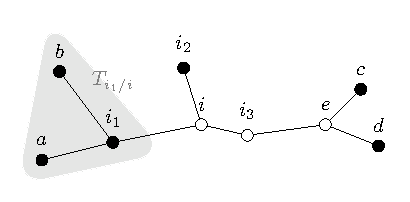
\includegraphics[scale=1.4]{figurer/objexp.eps}
  \caption{Example instance explaining power levels necessary for transmitting a signal from different sources}
  \label{fig:objexp}
\end{figure}


Consider an edge $\{i,j\}$ in a solution $T$ to SBT.
Let $T_{i/j}$ denote the subtree of $T$ consisting of nodes whose path to $j$ contains $(i,j)$. 
A node $i$ in $T$ contributes to the objective function by the expression $c_T(i)$ as follows:
\begin{equation}
c_T(i)=|T_{i_1/i}|p_{ii_2} + |T\setminus T_{i_1/i}|p_{ii_1}.
\end{equation}
We can also regard $c_T(i)$ as a weighted arithmetic mean of $i$'s power levels, with weights corresponding to the number of nodes whose signal is transmitted using the corresponding power level.
The objective function is to minimize overall nodes' contributions, that is,
\begin{equation}
c(T)=\sum\limits_{i\in V}c_T(i).
\label{eq:sbtcost}
\end{equation}
The problem under study is thus defined as follows:
\begin{problem}
Find a tree $T\subseteq G$ spanning $D$ minimizing \eqref{eq:sbtcost}.
\end{problem}

\emph{Remark:} The requirement that a solution must be a tree is necessary due to the nature of the objective function.

Like in MEB, an optimal solution to SBT does not guarantee a planarity of the resulting tree, although vast majority of instances are planar. 
As an example of non-planar optimum we state the instance on five nodes depicted in Fig~\ref{fig:sbtnonplanar}.
\begin{figure}[htb!]
  \centering
  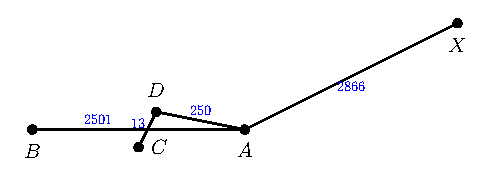
\includegraphics[scale=1.4]{figurer/sbtnonplanar.eps}
  \caption{A unique optimal solution with crossing to an instance of SBT with objective function value 19904. 
  If the arc $(DC)$ is forbidden, the optimal solution becomes a star graph with objective function value 19917.
  The nodes have coordinates $A=[50,30]$, $B=[49,80]$, $C=[51,48]$, $D=[48,46]$ and $X=[5,1]$.}
  \label{fig:sbtnonplanar}
\end{figure}

\subsection{Non-destination nodes}

Additional assumption of the existence of nodes that never initiate any transmission is a natural extension of all the problems described above.
It is similar to the generalization of MST which leads to the Steiner minimum tree problem.
In MEB, RAP and SBT, nodes that do not have to be part of the network are also allowed. 
These nodes never initiate any transmission, nor they have to receive any signal.
They can act as intermediate nodes relaying the signal, if improves the respective objective function value.
Apart from the weighted graph $G=(V,E,p)$, the set of nodes $D\subseteq V$ called \emph{destinations} is also a part of the input.
Nodes in $V\setminus D$ are referred to as \emph{non-destinations}.

In MEB, the presence of non-destinations leads to the Minimum Energy Multicast (MEM) problem introduced along with MEB in \cite{wieselthier00}.
It is easy to see that MEM is NP-hard by reducing the Steinter tree problem to it.


The following section gives a particular attention to the multicast version of SBT.

\section{Shared Multicat Trees}

The Shared Multicast Tree (SMT) problem is a natural generalization of SBT.
         % Introduction
\chapter{Minimum Broadcast Time}\label{sec:mbt}

Broadcasting is the information dissemination process in a communication network.
The Minimum Broadcast Time (MBT) problem is identified by a set of communication devices (nodes), among which some selected ones acts as an originators of a signal.
The number of originators is at least one, and we refer them as \emph{sources}.
The task is to spread a signal from the sources to the remaining nodes along the communication links defined by edges $E$ in a shortest possible time.
The continuous time is divided into discrete time steps.
The communication among the nodes must fulfill the following rules:
\begin{enumerate}
\item Each transmission takes place between two adjacent nodes
\item Each transmission requires one time step
\item Each node can participate in at most one transmission per one time step
\end{enumerate}

This communication protocol appears in various practical applications such as communication among computer processors and telephone networks.
In satellite networks, even though the communication is wireless, signals have to cover large distances, 
and so the information is sent from one satellite to one of its neighbours at a time.
The MBT problem was studied in the context of an existing Chinese BeiDou Global Navigation Satellite System~\cite{chu17}.

\section{Network Model and Definitions}

The communication network is determined by a graph $G=(V,E)$ and a subset $S\subseteq V$ of sources.

\begin{definition}\label{def:mbt}
The broadcast time $\tau(G,S)$ of $S\subseteq V$ in $G$ is defined as the smallest integer $t\geq 0$
for which there exists a sequence $V_0\subseteq\dots\subseteq V_t$ of node sets and a function $\pi:V\setminus S\mapsto V$, satisfying:
\begin{enumerate}
\item $V_0=S$ and $V_t=V$,
\item for all $v\in V\setminus S, \left\{v,\pi(v)\right\}\in E$,
\item for all $k=1,\dots t$ and all $v\in V_k$, $\pi(v)\in V_{k-1}$, and
\item for all $u,v\in V_k\setminus V_{k-1}$, $\pi(u)=\pi(v)$ only if $u=v$.
\end{enumerate}
\end{definition}
Any feasible solution determines a communication forest $\mathcal{F}$.
It is easily verified that the \emph{communication forest} contains arborescences rooted at distinct sources.
Individual arborescences in $\mathcal{F}$ are referred to as \emph{communication trees}.
Let $T_s=\left(V_{T_s},A_{V_s}\right)$ denote the communication tree rooted at source $s\in S$, and define the function $\alpha:V\to S$ such that $v\in V_{T_{\alpha(v)}}$ for all $v\in V$.
That is, $\alpha$ associates a node $v$ with the source at which the communication tree containing $v$ is rooted.
For an arc $(i,j)$ in a given communication tree, the integer $t_{i,j}$ denotes the time step in which node $i$ informs $j$.
%For any communication tree $T_s$, let $T^i_s$ be the subtree of $T_s$ induced by the set of nodes with distance at most $i$ edges from $s$.
%Analogously, let $D^i=\left\{T_s^i: s\in S\right\}$.

Formally, the optimization MEB problem is defined as follows:
\begin{problem}\label{mbt:opt}
Given $G=(V,E)$ and $S\subseteq V$, find $\tau(G,S)$. 
\end{problem}
In the literature, authors often consider the decision version, because some of the theoretical results depend on a given time limit.
\begin{problem}\label{mbt:dec}
Given $G=(V,E)$, $S\subseteq V$,  and a time limit $t\in \mathbb{Z}^+_0$, does $\tau(G,S)\leq t$ hold? 
\end{problem}

The \emph{broadcast center} of a graph is the set of all nodes having the smallest broadcast times ,i.e., $\arg\min\left\{\tau(G,\{v\}):v\in V\right\}$.
%\section{Problem Definition}

%\section{Broadcast Graphs}

\section{Computational Complexity}

MBT has been thoroughly studied from the perspective of computation complexity and approximability, particularly in the early 90'.
ITS NP-completeness or belonging to P was shown for various graph classes and values of time limit $t$.

It has been shown that the problem is NP-complete for arbitrary graphs in \cite{garey79} and few years later, 
this result was obtained for arbitrary graphs with deadline $t=4$ and a single source by reduction from \textsc{3D Matching}~\cite{slater81}. 
The same work also contains a $\mathcal{O}(n)$ algorithm for determining broadcast time of a tree with a single source. 
As a by-product, this algorithm determines the broadcast center of the input tree.

These results are improved and extended in~\cite{jansen93}, where the authors exploit the properties of NP-complete problem \textsc{Planar 3-SAT}.
First, they prove that \textsc{Planar 3,4-SAT} is NP-complete, and subsequently use this property to show that MBT is NP-complete for:
\begin{itemize}
\item bipartite planar graphs, deadline $t=2$ and maximum degree at most 3,
\item split graphs with deadline $t=2$,
\item chordal graphs with a single source, 
\item planar graphs with single source and maximum degree at most 3, 
\item bipartite planar graphs with maximum degree at most 3 and a single source,
\item grid graphs with deadline $t=2$ and maximum degree at most 3,
\item grid graphs with a single source, and
\item complete grid graphs with deadline $t=2$. 
\end{itemize}
The question whether MBT is NP complete for split graphs with a single source is stated as open.
Another complexity result proving that MBT remains NP-complete for 3-regular planar graphs with constant deadline $t\geq 2$ 
is given in \cite{middendorf93} by reduction from \textsc{Exactly-one-in-three-3-SAT}.

The complexity results above typically exploit sophisticated reductions.
We provide a very simple and straightforward proof of NP-completeness of MEB for time limit at most $t=3$ on graphs with maximum degree at most 3.
There are many restrictions on SAT that preserve NP-completeness.
We concentrate on the variant of 3-SAT with the property that each variable is restricted to appear at most three times, and each literal at most twice. 
This problem is known as 3-3-SAT, and its NP-completeness proof can be found in~\cite{papadimitriou94}. 
Note that in this particular version of 3-SAT, it can no longer be assumed that each clause consists of exactly 3 literals.
Further, the assumption about at most two occurrences of a literal is automatic, 
because formula $\varphi$ that contains a variable $x$ that appears only as a positive or only as a negative literal can trivially be transformed into $\varphi'$ that does not contain $x$ at all, 
such that $\varphi$ is satisfiable if and only if $\varphi'$ is satisfiable.
\begin{lemma}\label{lemma:mbtred}
Let $\varphi$ be an instance of \textsc{3-3-SAT}, and let $G=(V,E)$ and $S\subseteq V'$ be an instance of MEB constructed from $\varphi$. 
Then, $\varphi$ is satisfiable if and only if $\tau(G,S)\leq 3$.
\end{lemma}
\begin{proof}\label{prop:mbtnpc}
An instance of Problem \ref{mbt:dec} is constructed from an instance $\varphi(x_1,\dots,x_n)$ of \textsc{3-3-SAT} as follows.
For each variable $x_i$ $\varphi$, we construct a gadget comprising five $x_i$, $\bar{x}_i$, $u_i$, $v_i$, $w_i$, where $u_i$ is a source, $i=1,\dots n$ .
The first two nodes represent possible literals associated with the variable $x_i$.
The gadget further contains four edges, $\{u_i,x_i\}$, $\{u_i,\bar{x}_i\}$, $\{u_i,v_i\}$, and $\{v_i,w_i\}$.
For each clause $c_j$, there is a node $c_j$ and whenever the clause $c_j$ contains a literal $x_i$ ($\bar{x}_i$), there is an edge $\{c,x_i\}$ ($\{c,\bar{x}_i\}$).
%We therefore have clause nodes of degree at most 3, because $\varphi$ is in 3-CNF.
%Nodes representing literals are connected to at most two clause nodes, which is implied by the restriction imposed on $\varphi$.
Using this construction we show the equivalence as the lemma states.

Let $\varphi$ be satisfialbe.
A source node $u_i$ sends the signal towards the node representing literal that is evaluated as true in the given truth assignment.
In the next time steps, the signal is further relayed to the node representing clause that is satisfied by the literal.
As each literal can cause satisfaction of up to two clauses, the corresponding clause nodes receive the signal from the respective literals within the time limit 3.
Nodes $u_i$ must receive the signal in the time step 2, in order to reach $w_i$ on time.
Thus, the node representing literal evaluated as false receives the signal in time step 3.

Conversely, let the constructed instance of MBT have broadcast time less than 3.
In a solution $T$ to the instance (highlighted as blue)  $\arg\min_{v\in\{x,\bar{x}\}}\{t_{u_x,v}\}$ represents the assignment of truth value to the variable $x$.
The presence of an arc entering a clause node $c$ in $T$ indicates that a truth value of certain variable caused satisfaction of clause $c$.
%The truth evaluation of clauses can be retrieved by looking up nodes representing literals that receive the signal in time step 1.
The auxiliary path $(u_x,v_x,w_x)$ ensures that the clause satisfaction is modeled correctly.
As $t_{u_x,v_x}\leq 2$, one of $t_{u_x,x}$ and $t_{u_x,\bar{x}}$ must be 3, 
and thereby the arc that would incorrectly indicate satisfaction of a clause that is not satisfied by the selected truth assignment would have cost 4, which is not allowed.
It is possible to have an arc outgoing from a clause node of cost 3, but the second endpoint is always a node representing some literal $y$, but the arc $(u_y,y)$ is already a part of $T$.

The correctness of the truth valuation is ensured by the existence of nodes $v_i$, so that the node representing literal that is evaluated as false is informed in time step 3, 
and thereby cannot forward the signal to any clause nodes.
\end{proof}

For illustrating the construction in proof of Prop.~\ref{prop:mbtnpc}, consider the following instance of \textsc{3-3-SAT}
\begin{equation}
\varphi=(x_1\vee x_2\vee x_3)\wedge(\bar{x}_1\vee x_4)\wedge(x_2\vee \bar{x}_3 \vee\bar{x}_4)\wedge(\bar{x}_1\vee \bar{x}_3)\wedge \bar{x}_2 
\label{eq:phi}
\end{equation}
reducing to the instance of Problem \ref{mbt:dec} depicted in Fig. \ref{fig:mbtnpc}.
\begin{figure}
\centering
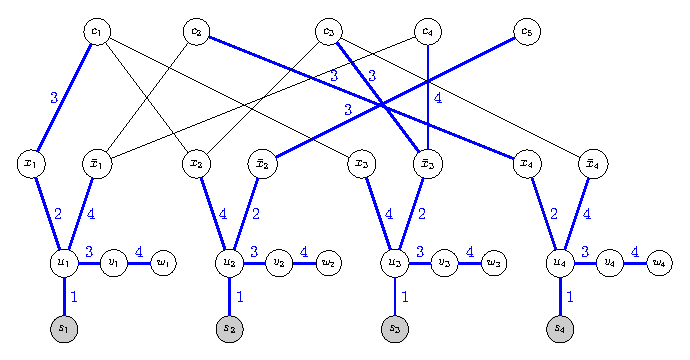
\includegraphics{figurer/mbtnpc.eps}
\caption{Reduction from formula $\varphi$ (Eq.~\eqref{eq:phi}) of \textsc{3-3-SAT} to an instance of MBT with deadline 4 and maximum node degree 4}
\label{fig:mbtnpc}
\end{figure}

\begin{proposition}
MBT is NP-complete for graphs with maximum node degree 4 and deadline 4.
\end{proposition}
\begin{proof}
In \cite{slater81}, a polynomial algorithm for MBT in trees is devised.
As the sequence of vertices $V_0\subseteq\dots\subseteq V_t$ and function $\pi$ in Def.~\ref{def:mbt} determine a unique forest of arborescences $\mathcal{F}$,
it can be verified in polynomial time whether the broadcast time of each braodcast tree in $\mathcal{F}$ does not exceed 3, proving that MBT belongs to NP.
This concludes together with Lemma~\ref{lemma:mbtred} that MBT is NP-complete for deadline at most 3.

It remains to show that the problem remains NP-complete for graphs with maximum degree bounded by 3.
As each literal appears at most twice in $\varphi$, the degree of nodes representing literals is at most 3. 
Each clause node has degree at most 3 since $\varphi$ is in 3-CNF.
Degrees of nodes $u_i$, $v_i$, and $w_i$ do not depend on $\varphi$, and have degrees 3, 2, and 1, respectively.
Thus, none of the node degrees in the constructed MBT instance exceeds 3.
\end{proof}

\section{Integer Linear Programming Models}

A straightforward ILP formulation has been proposed in Paper IV together with a suitable solution method.
A similar formulation has been recently published in \cite{mbtheurXX}.
ILP formulation of the problem of \textsc{Minimum Broadcast Graph} are studied in \cite{McGarvey16}.
The authors focus on the $c$-broadcasting  and $k$-fault-tolerant $c$-broadcasting variants of the problem.

In the following, we present an unpublished ILP model for MBT.

\subsection{Binomial Tree Model}

A binomial tree $B^k$ of order $k$ is an ordered tree defined recursively as follow \cite{cormen01}:
\begin{itemize}
\item The binomial tree $B^0$ consists of a single node.
\item The binomial tree $B^k$ has a root with $k$ children where the $i$-th child is the root of a binomial tree of order $k-i$, $i=1,\dots,k$.
\end{itemize}
An example of $B^3$ is depicted in Fig.\ref{fig:beta}.
%If a solution to MBT consists of broadcast trees that are binomial, the number of informed nodes doubles in each time step.
For a given time step $k$, the maximum number of informed nodes within $k$ steps is $|S|2^k$.
This occurs when the solution of MBT consists of broadcast trees that are binomial.
%Any broadcast tree can be regarded as pruned binomial tree.
%Problem \ref{prob:min} can therefore be restated as finding a partition of $G$ into $m$ pruned binomial trees
\begin{observation}
\label{obs:btspread}
if $r$ is the root of $B^k$, then $\tau(B^k,\{r\})=k$.
\end{observation}
\begin{figure}
\centering
	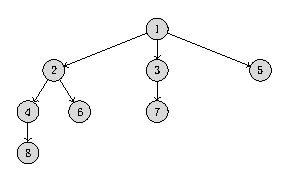
\includegraphics{figurer/btindex.eps}
\caption{A binomial tree with nodes labeled by their positions}
\label{fig:beta}
\end{figure}

\subsubsection{Binomial trees over positive integers}

Let $k\in \mathbb{N}$ and $I=\{1,\dots,2^k\}$.
A directed binomial tree $B^k=(V_{B^k},A_{B^k})$ with arcs oriented towards the leaves has a regular structure that allows to define a systematic numbering of nodes so that a node number determines unambiguously a position in $B^k$.
That is, we need an applicable bijective function $\beta:V_{B^k}\to I$.
A suitable bijection $\beta$ assigns values from $I$ to nodes increasingly with decreasing outgoing degree.
If there is an ambiguity, a node whose parent has a lower number is assigned a lower number.
This function is defined recursively as
\begin{equation*}
\label{eq:beta}
\beta(v)=\begin{cases}
1,\text{ if } v \text{ is the root of } B^k,\\
\beta(u) + 2^{k-deg^+(v)-1}, (u,v)\in A_{B^k},\text{ otherwise}.
\end{cases}
\end{equation*}
Nodes in Fig. \ref{fig:beta} are labeled with their $\beta$-values.
Pairs of integers that are assigned to adjacent nodes in a binomial tree are defined by relation
\begin{equation*}
\label{eq:betarel}
R=\{(i,j)\in\mathbb{N}\times\mathbb{N}:j=i+2^k,k\geq\log i,k\in \mathbb{Z}\}.
\end{equation*}

We further define the function $\pi':\mathbb{N}\to\mathbb{Z}_+$ that for a given integer $i$ associated with node $v$
determines $\beta$-value of parent of $v$:
\begin{align*}
\label{eq:piprime}
\pi'(1)&=0,& \\
\pi'(j)&=j-2^{\lceil\log j\rceil -1}, &j > 1.
\end{align*}
Using functions $\alpha$, $\beta$, $\pi'$ and the relation $R$, we introduce the notion of binomial trees over positive integers.
\begin{definition}
A pair $(I,X)$ where $I=\{1,\dots,2^k\}$, $k\in\mathbb{Z}_+$, $(\alpha(u),\beta(u))=(\alpha(v),\beta(v))\Leftrightarrow u=v$ and
$X=\{(i,j)\in R, i,j\in I\}$ is an \emph{integer binomial tree of order $k$}.

$(I,X)$, where $I\subseteq\{1,\dots,2^k\}, k\in \mathbb{Z}_+,\pi(j)\in I$ for all $j\in I\setminus\{1\}$ and
$X=\{(i,j)\in R, i,j\in I\}$ is an \emph{integer binomial tree of order $k$ pruned at $\{1,\dots,2^k\}\setminus I$}.
\end{definition}
We now develop a method for modelling Problem \ref{mbt:opt} whose main principle is finding a partition of $G$ into pruned binomial trees.
For any integer $i$, let $I_i=\{2^{i-1}+1,\dots,2^i\}$.
%\begin{problem}
%\label{prob:dec}
%Given $G=(V,E)$, $S\subseteq V$ and $t\in \mathbb{N}$, is there a sequence $S=V_0\subseteq\dots\subseteq V_t=V$
%and a mapping $\pi:V\setminus S\to V$, such that for each $v\in V\setminus S:\{v,\pi(v)\}\in E$ and for each  $u,v\in V_i\setminus V_{i-1}: \pi(u)\neq \pi(v)\Leftrightarrow u\neq v$?
%\end{problem}
%For a delay $t$, at most $s\cdot 2^t$ nodes can be informed within $t$ steps.
%Therefore, we assume $n\leq 2^ks.
%This can be achieved when the broadcast forest $T$ consists of binomial trees $B^t$ of order $t$ rooted at sources $s\in S$.
%Hence, if there is a partition of $G$ into $s$ pruned binomial trees of order at most $t$ rooted at sources, then $(G,S,t)$ is a YES instance of Problem \ref{prob:dec}.
%Finding a partition of $G$ into $s$ pruned binomial trees can be equivalently formulated as finding a partition of $G''$ into $s$ (complete) binomial trees,
%where $G''$ is constructed from $G$ as follows:
%Let $\alpha\coloneqq s\cdot 2^k-|V|$, and let $K_\alpha=(V_\alpha,E_\alpha)$ be a complete graph on $\alpha$ nodes.
%Each node in $K_\alpha$ is connected to every node $v\in V$ in the original graph $G$.
%Thus, $G''=(V'',E'')$ with $V''=V\cup V_\alpha$ and $E''=E\cup E_\alpha\cup \{\{u,v\}: u\in V \wedge v\in V_\alpha\}$.
%The set of arcs $A''$ is constructed by creating two arcs of opposite orientation for each edge, but arcs with orientation from $V_\alpha$ to $V$ are excluded.
%Formally, $A''=A\cup\{(u,v),(v,u): \{u,v\}\in E_\alpha\}\cup\{(u,v):u\in V \wedge v\in V_\alpha\}$.

%\begin{observation}\label{obs:deg}
%For each $i\in\{1,\dots,t\}$, the set $\{v\in V^t: 1\leq\beta(v)\leq2^i\}\setminus\{v\in V^t:1\leq\beta(v)\leq2^{i-1}\}$ contains nodes with out-degree $t-i$.
%\end{observation}
%\begin{observation}\label{obs:childdeg}
%Children of $v\in V^t$ with $\text{deg}^+(v)=\ell$ have out-degree $0,\dots,\ell-1$.
%\end{observation}
\begin{observation}\label{obs:eqbetalevel}
$\pi'$ is injective.
%For $i_1,i_2\in I_i$, $\pi'(i_1)=\pi'(i_2)\Leftrightarrow i_1=i_2$.
\end{observation}
\begin{proof}
We notice that $\lceil\log (2^{i-1}+1)\rceil=\dots =\lceil\log 2^i\rceil$, and thus $\pi'(2^{i-1}+1),\dots,\pi'(2^i)$ are pairwise different.
\end{proof}

\begin{proposition}\label{lem:probeq}
A graph $G=(V,E)$ and $S\subseteq V$ has $\tau(G,S)\leq k$ iff it is possible to assign integers to nodes
such that they form $m$ (pruned) integer binomial trees of order $k$ or smaller rooted at sources.
\end{proposition}
\begin{proof}
Assume nodes in $V$ can be labeled by integers from $I=\{1,\dots,2^k\}$ so that they form (pruned) integer integer binomial trees $B_\ell$ of order at most $k$, $1\leq\ell\leq m$.
For $r\in V_{B_\ell}$ with $\alpha(r)=r$ and $\beta(r)=1$, by Obs. \ref{obs:btspread}, $\tau(B_\ell,\{r\})\leq k$.
The sequence of node sets $V_0,\dots,V_k$ is constructed by setting $V_0=\{v\in V:\beta(v)=1\}$, and $V_{i}=V_{i-1}\cup\{v\in V: \beta(v)\in I_i\}$.
Moreover, $\pi(v)=u\Leftrightarrow \alpha(v)=\alpha(u)~\&~\pi'(\beta(v))=\beta(u)$.
Also, $\pi(u)=\pi(v)\Leftrightarrow u=v$ follows from Obs. \ref{obs:eqbetalevel}, because nodes in $V_i$ have $\beta$ values in $I_i$.

Conversely, suppose there is a sequence of subsets and a function $\pi$ in $G$ with the desired properties.
Nodes are associated with integers from $I$ assigned according to the following steps:
\begin{enumerate}
\item $\beta(s)=1$ for all $s\in V_0$,
\item For $v\in V_i$, set $\beta(v)=j$ such that $j\in I_i$ and $(\pi'(\beta(v)),j)\in R, 1\leq i\leq k$.
\end{enumerate}
\qed
\end{proof}
\subsubsection{The formulation}
Consider a graph $G'=(V',E')$ constructed  by adding a universal node $v_0$ to $G$.
The set of nodes and edges is then $V'=V\cup \{v_0\}$ and $E'=E\cup\{\{v_0,v\}:v\in V\}$.
Apart from $z$-variables introduced in model \eqref{mod:basic}, the ILP formulation based on partition into binomial trees uses
$$
y_{is}^v=\begin{cases}
1, \text{ if } \beta(v)=i \text{ and } \alpha(v)=s,\\
0, \text{ otherwise},\\
\end{cases}
$$
where $v\in V'$, $i\in I$, $s\in S$ and $0\leq j\leq \bar{t}$.
With the definition of $G'$ above, it is straightforward to specify constraints that enforce desired values for $y$-variables.
Whenever $y_{is}^{v_0}=1$, it indicates that the binomial tree rooted at $s$ is pruned at node with position $i$.
%An obvious weakness of this approach is  that the number of nodes increases to $|V''|=\mathcal{O}(ns)$, and the dimension of variables is thus $\mathcal{O}(n^2s^2)$.
%However, once a suitable partition is found, the arcs of binomial trees contained in $K_\alpha$ can be diversely shuffled while preserving the layour of binomial trees in $G$.
%Instead of adding the entire complete graph $K_\alpha$, a single node $v_0$ with a loop $(v_0,v_0)$ is connected as an apex to the original $G$.
%Let us denote this multigraph as $G'=(V',E')$, where $V'=V\cup\{v_0\}$, $E'=E\cup\{\{u,v_0\}:u\in V\}\cup\{\{v_0\}\}$.
%The arc set is then analogously defined as $A'=A\cup\{(u,v_0): u\in V\}\cup\{(v_0,v_0)\}$.
%The requirement for partition into binomial trees has to be adjusted accordingly.
%The subtrees contained in $G$ remain unchanged, every arc $(u,v)\in A^k_i, i=1,\dots,s$ in $G''$ with $u\in V$ and $v\in V_\alpha$ becomes $(u,v_0)$ in $G'$,
%and every $(u,v)\in A_\alpha$ becomes $(v_0,v_0)$.
%So, $v_0$ acts as a universal node that can substitute several nodes in each binomial tree.
Let us define the set $C(i)$ of $\beta$-positions of children (direct descendants) of node $v$ with $\beta(v)=i$ in a binomial tree of order $k$:
\begin{equation}
\label{eq:c1}
C(i)=\{2^j+i:j=\lceil\log_2 i\rceil,\dots,k-1\}.
\end{equation}
The formulation based on binomial trees is the following:
\begin{subequations}\label{mod:partition}
\begin{align}
\notag &\min\sum\limits_{j=0}^{\bar{t}}z_j,\\
\notag \text{s. t. } \\
\label{mod:part:nodeBelongs} \sum\limits_{i\in I}\sum\limits_{s\in S}y^v_{is} & = 1 & v\in V,\\
\label{mod:part:treeHasIJ} \sum\limits_{v\in V'}y^v_{is} & = 1 & i\in I,s\in S,\\
\label{mod:part:source1} y_{1s}^s & = 1  & s\in S,\\
%\label{mod:part:noReturn} y^u_{ij}+y^v_{lj} &\leq 1 & i\in I,l\in C(i), j\in J, u\in V_\alpha,v\in V,\\
%\label{mod:part:followArcs} y^u_{is}+y^v_{\ell s} &\leq 1 & i\in I,\ell\in C(i), s\in S, u,v\in V',(u,v)\not\in A',\\
%\label{mod:part:followArcsA} y^u_{is}+y^v_{\ell s} &\leq 1 & i\in I,\ell\in C(i), s\in S, u,v\in V,\{u,v\}\not\in E,\\
%\label{mod:part:followArcsB} y^{v_0}_{is}+y^v_{\ell s} &\leq 1 & i\in I,\ell\in C(i), s\in S, v\in V,\\
%\label{mod:part:followArcsA}y^{v_0}_{is}+y^u_{i s} + \sum\limits_{v\in V\setminus N(u)}y^v_{\ell s}&\leq 1 & u\in V,i\in I,\ell\in C(i), s\in S,  \\
%\label{mod:part:followArcsB}y^{v_0}_{is}+y^u_{\ell s} + \sum\limits_{v\in V\setminus N(u)}y^v_{i s}&\leq 1 & u\in V,i\in I,\ell\in C(i), s\in S,\\
\label{mod:part:followArcsA}\sum\limits_{v\in \bar{N}(u)}y^v_{\ell s}&\leq \sum\limits_{v\in N(\bar{N}(u))}y_{is}^{v} & u\in V,i\in I,\ell\in C(i), s\in S,  \\
\label{mod:part:followArcsB}\sum\limits_{v\in \bar{N}(\bar{N}(u))}y^v_{\ell s}&\leq \sum\limits_{v\in N(u)} y_{is}^{v} & u\in V,i\in I,\ell\in C(i), s\in S,\\
\label{mod:part:yzrel}\sum\limits_{v\in V}y^v_{is} & \leq z_{\lceil\log i\rceil} & i\in I,s\in S,\\
\label{mod:part:dim}&&y \in \{0,1\}^{I\times S\times V'}, z\in \{0,1\}^{\bar{t}}.
\end{align}~
\end{subequations}

%As the model represents the decision problem, it suffices to find any feasible solution, and no objective function is needed.
The interpretation of constraints \eqref{mod:part:nodeBelongs} is that every node in the original graph $G$ belongs to exactly one binomial tree.
Note that these constraints are quantified only over $V$ and not over $V'$.
In this way it is achieved that $v_0$ can be regarded as a part of several binomial trees.
By \eqref{mod:part:treeHasIJ} is ensured that exactly one node, possibly $v_0$, is allocated to position $i$ of each binomial tree.
By the summation over $V'$ is ensured, that pruned nodes are collectively represented by $v_0$.
Next, \eqref{mod:part:source1} enforce that source nodes are always the first nodes in corresponding binomial trees, in accordance with definition \eqref{eq:beta} of the function $\beta$.
The remaining two sets of constraints guarantee that the arcs of binomial trees follow edges in $E$.
%In particular, it is enforced by \eqref{mod:part:followArcsA} that if $u$ and $v$ are not adjacent in $G$, then $v$ must not act as a child of $u$ in any binomial tree.
In particular, it is enforced by \eqref{mod:part:followArcsA} that if there is some  non-neighbor $v$ of $u$  with a label $\ell$ in a binomial tree rooted at $s$,
then there must be a neighbor of some non-neighbor of $u$ with label $i$ in the same binomial tree.
Similarly, Constraints \eqref{mod:part:followArcsB} state that if there is a node $v$ with label $\ell$ in a binomial tree rooted at $s$ in the complement of neighborhood of all non-neighbors of $u$,
there must also be a neighbor of $u$ with label $i$ in this binomial tree.
This reflects the obvious fact that if a tree is pruned at some node, all its descendants must also be excluded from the tree.
%The definition of $A'$ also prevents arcs of the binomial trees to be oriented from $V_\alpha$ to $V$.
%In other words, once the signal leaves the original graph $G$ and enters $v_0$, it cannot return back to $G$.
Without \eqref{mod:part:followArcsA} and \eqref{mod:part:followArcsB}, it could be possible to find a feasible solution, even when no partition of $G$ into pruned binomial trees exists.
Finally, the relation \eqref{mod:part:yzrel} between $y$ and $z$ variables follows from Obs. \ref{obs:btspread}.
It says that whenever there is a node in a position $i$, then the delay is at least $\lceil\log i\rceil$.
%Constraints \eqref{mod:part:followArcsA} and \eqref{mod:part:followArcsB} can be replaced by stronger
%\begin{subequations}
%\begin{align}
%\label{mod:part:followArcsAStrongerA}
%y^{v_0}_{is}+y^u_{i s} + \sum\limits_{v\in V\setminus N(u)}y^v_{\ell s}&\leq 1 & u\in V,i\in I,\ell\in C(i), s\in S,  \\
%\label{mod:part:followArcsAStrongerB}
%y^{v_0}_{is}+y^u_{\ell s} + \sum\limits_{v\in V\setminus N(u)}y^v_{i s}&\leq 1 & u\in V,i\in I,\ell\in C(i), s\in S.
%\end{align}
%\end{subequations}
%
\subsubsection{Valid inequalities}
Let $W$ be a maximal independent set in $G$.
Model \eqref{mod:partition} is strengthened by
\begin{align}
\label{mod:part:vibasic}
y^{v_0}_{is}+ \sum\limits_{v\in W}(y^v_{is}+y^v_{\ell s})&\leq 1 & i\in I,\ell\in C(i), s\in S,
\end{align}
which exploits the fact that no pair of nodes in $W$ is adjacent, and so there must be no two nodes with adjacent $\beta$-positions.

We now generalize this idea by using the notion of graph power $G^m=(V,E^m)$ commonly defined as a graph with the same set of nodes as $G$,
and an edge between two nodes in $G^m$ is present iff there is a path of length at most $m$ between them in $G$.
For our purposes, we use a slightly modified definition of the edge set
$$E^m=\{\{u,v\}:\text{there exists a path between $u$ and $v$ in $G$ of length $m$}\}.$$
Definition \eqref{eq:c1} can be generalized to descendants of an arbitrary distance $m$ from $v$ in $B^k$:
\begin{equation}
C^{m+1}(i)=\bigcup_{j\in C^1(i)}C^m(j).
\end{equation}
For a given $m$, let $W_m$ be a maximal independent set in $G^m$.
Further strengthening of model \eqref{mod:partition} is achieved by introducing valid inequalities
\begin{align}
\label{mod:part:vigeneral}
y^{v_0}_{is}+ \sum\limits_{v\in W_m}(y^v_{is}+y^v_{\ell s})&\leq 1 & i\in I,\ell\in C^m(i), s\in S,1\leq m\leq \Delta_G-1.
\end{align}
Clearly, inequality \eqref{mod:part:vibasic} is included in \eqref{mod:part:vigeneral} for $m=1$.
The distance between positions $i$ and $\ell=C^m(i)$ in a binomial tree is $m$.
The maximal independent set $W_m$ contains nodes such that length of any path between any two nodes is different from $m$,
and so there must not be two nodes in $W_m$ with positions $i$ and $\ell$ at the same time.

\subsubsection{Symmetry removal}
Another improvement of this model is achieved by a symmetry removal.
If a broadcast tree is identical to a binomial tree, we notice that nodes with labels from $C(i)$, i.e., children of some node $v$ with $\beta(v)=i$, are informed in increasing time steps.
For example in $B^3$, $C(2)=\{4,6\}$ and the corresponding nodes are informed in time step 2 and 3, respectively.
If a label $\ell\in C(i)$ corresponds to a node of a binomial tree that is pruned (if $y^{v_0}_{\ell s}=1$ for some $s\in S$),
all labels $j\in C(i)$ such that $j>\ell$ can also be pruned.
Thus, adding
\begin{align}
\label{mod:part:sr}
y^{v_0}_{js}&\leq y^{v_0}_{\ell s}&i\in I,j,\ell\in C(i),j<\ell, s\in S
\end{align}
to the model reduces the set of feasible solutions.

\subsubsection{Decision version}

In a similar manner as we derived the decision version \eqref{mod:basic:dec} of model \eqref{mod:basic}, it is possible to construct a decision version of the binomial tree model \eqref{mod:partition} as follows:
\begin{subequations}\label{mod:genmatch}
\begin{align}
\notag \max\sum\limits_{v\in V}&\sum\limits_{i\in I}\sum\limits_{s\in S}   y_{is}^v,\\
\notag \text{s. t. } \\
\label{mod:genmatch:nodeBelongs} \sum\limits_{i\in I}\sum\limits_{s\in S}y^v_{is} & \leq 1 & v\in V,\\
\notag\eqref{mod:part:treeHasIJ} - \eqref{mod:part:followArcsB},\\
%\label{mod:genmatch:treeHasIJ} \sum\limits_{v\in V'}y^v_{is} & = 1 & i\in I,s\in V_T,\\
%\label{mod:genmatch:source1} y_{1s}^s & = 1  & s\in V_T,\\
%\label{mod:part:noReturn} y^u_{ij}+y^v_{lj} &\leq 1 & i\in I,l\in C(i), j\in J, u\in V_\alpha,v\in V,\\
%\label{mod:part:followArcs} y^u_{is}+y^v_{\ell s} &\leq 1 & i\in I,\ell\in C(i), s\in S, u,v\in V',(u,v)\not\in A',\\
%\label{mod:part:followArcsA} y^u_{is}+y^v_{\ell s} &\leq 1 & i\in I,\ell\in C(i), s\in S, u,v\in V,\{u,v\}\not\in E,\\
%\label{mod:part:followArcsB} y^{v_0}_{is}+y^v_{\ell s} &\leq 1 & i\in I,\ell\in C(i), s\in S, v\in V,\\
%\label{mod:genmatch:followArcsA}y^{v_0}_{is}+y^u_{i s} + \sum\limits_{v\in V\setminus N(u)}y^v_{\ell s}&\leq 1 & u\in V,i\in I,\ell\in C(i), s\in V_T,  \\
%\label{mod:genmatch:followArcsB}y^{v_0}_{is}+y^u_{\ell s} + \sum\limits_{v\in V\setminus N(u)}y^v_{i s}&\leq 1 & u\in V,i\in I,\ell\in C(i), s\in V_T,\\
\label{mod:genmatch:dim}&&y \in \{0,1\}^{I\times S\times V'}.
\end{align}~
\end{subequations}
This model is a modification of formulation \eqref{mod:partition}, and uses the same type of variables.
The objective function is to maximize the number of nodes involved in the binomial trees.
In order to determine the minimum broadcast time, we are looking for the minimum $k$ such that each node can be assigned a label from the set $I=\{1,\dots,2^k\}$ while satisfying given constraints.
%The index set $I=\{1,\dots,2^k\}$ depends on the input parameter $k$.
The constraints \eqref{mod:genmatch:nodeBelongs} state that each node belongs to at most one binomial tree.
Compared to \eqref{mod:part:nodeBelongs}, \eqref{mod:genmatch:nodeBelongs} is an inequality, because the binomial trees do not necessarily form a partition of $G$, and so not all nodes have to be used.
The remaining constraints are taken from formulation \eqref{mod:partition}.

The approach is then analogous to the idea indicated in Section \ref{sec:decbasic}.
Assume we are given a lower bound $\underline{t}$ and an upper bound $\bar{t}$ on the minimum broadcast time.
Initially, we define the set $I=\{1,\dots,2^{\underline{t}}\}$ and iteratively solve the model while doubling the set $I$ until the objective function attains the value $n$.
That indicates that it is the first iteration in which all nodes are assigned a label, and it can be concluded that the minimum broadcast time is $\log_2|I|$.

%An objective function is naturally lacking in the formulation of the decision problem.
%It is nevertheless straightforward to create an ILP model for the corresponding optimization problem.
%Let $z_i=1 \Leftrightarrow t=i$ be a new variable and let $\bar{t}$ be an upper bound on the delay in $(G,S)$.
%Problem \ref{prob:min} is formulated as follows:
%\begin{subequations}
%\begin{align}
%\notag &\min\sum\limits_{j=0}^{\bar{t}}z_j,\\
%\notag \text{s. t. } \\
%\notag \eqref{mod:part:nodeBelongs} - \eqref{mod:part:source1},& \eqref{mod:part:followArcsAStrongerA} - \eqref{mod:part:followArcsAStrongerB}, \eqref{mod:part:vi}, \eqref{mod:part:sr},\\
%\notag\sum\limits_{v\in V}y^v_{is} & \leq z_{\lceil\log i\rceil} & i\in I,s\in S,\\
%\notag\label{mod:part:optdim}y &\in \{0,1\}^{I\times S\times V'}, z \in \{0,1\}^{\bar{t}}.
%\end{align}~
%\end{subequations}


Our preliminary experiments indicate that the published model in Paper IV determines an optimal solution faster, we believe that there is a room for improvement 


\section{Inexact Algorithms}

A number of heuristics methods as well as approximation algorithms along with associated theoretical results have been developed.

         % Introduction
\chapter{Multi-Agent Path Finidng}\label{sec:app}

In multi-robot path finding (MPF) we consider an environment with several identical moving entities referred to as 
\emph{agents}. Source and target locations are uniquely determined for each agent. The objective
is to find a route for every agent from its source to its target.
Agents must not collide with obstacles and other agents that are also moving along
planned routes towards their own targets.
The environment is modeled as an undirected graph, where the agents are placed in the vertices, and move along the edges from one vertex to another. 
Continuous time is divided into discrete time steps, where the relocation of an agent from one vertex to its neighbor takes exactly 1 time step.

Different variants and restrictions have been studied.

\emph{Muliti-agent path-finding} (MPF) \cite{source1}  supposes a group of agents in a given
environment, where initial and target positions are determined for each agent.
All individual agents must avoid collisions. Movement of the agents is carried
out in discrete time steps. Agent can shift from one vertex to its neighbor on
condition that the neighbor is either unoccupied or is being left by other agent
in the same time step. At most one agent is allowed to pass an edge within one
time step. That is, agents are not allowed to exchange their positions within one
time step.

\emph{Pebble motion on graphs} \cite{source1,source2} is a very similar problem as MPF. It can
be regarded as a restricted variant of MPF. The difference consists in rules for
movement. While MPF enables entering a vertex that is simultaneously being
left by other agent, such transfer is not permissible in pebble motion. As an
illustration we can mention 15 puzzle also known as Lloyd’s 15 \cite{lloydXX}.

\emph{Cooperative Path-finding} \cite{cpf} is a special case of MPF where each agent is
assumed to have a full knowledge of all other agents and their planned routes.
Precisely speaking, solving algorithm can take into account paths planned for
agents that were processed earlier, and adjust paths searched later according to
them.

\section{Scenarios with adversaries}

\subsection{Adversarial Cooperative Path Finding}

\subsection{Area Protection Problem}

\subsection{Area Protection Problem with Communication maintenance}

         % Introduction
%
% Modified mathematics bibliography. Uses acm.bst
%
\bibliographystyle{acm}

\bibliography{thesis}

\chapter{Contribution of the Thesis and Prospective Research}

This thesis is a compilation of six papers in which three independent topics are looked into.
The first three papers are focused on ad-hoc wireless networks discussed in Chapter~\ref{chap:wanet}.
The fourth paper deals with the broadcast time problem addressed in Chapter~\ref{chap:mbt}.
These four papers share the common characteristic that integer programming is an essential solution method.
In this sense, the last two papers are distinguished from the former.
They are devoted to adversarial variants of path finding for multiple robots summarized in Chapter~\ref{chap:app}, 
which are commonly approached by methods prevalent in the field of artificial intelligence.
%
% Paper I
%
\section{Paper I:  Shared Multicast Trees in Ad-hoc Wireless Networks}

The contribution of Paper I lies in introducing the Shared Multicast Tree (SMT) problem, a generalization of the Shared Broadcast Tree (SBT) problem.
An ILP model for SMT is proposed by modification of a model for SBT presented in \cite{yuan12}.
Additional constraints related to non-destination nodes are included in the model, and constraints in the existing model for SBT are quantified with respect to the non-destinations.
The presented model is subsequently proved to be a correct formulation of SMT.
Appendix A of Paper I contains details of the proof.

Further, several inexact construction methods are proposed.
The first two methods are based on construction of a solution to different problems, specifically MST and MEB, respectively. 
The construction is followed by local search, which identifies non-destinations whose presence in the solution is disadvantageous.
These non-destinations are then eliminated from the solution.
The third method is an algorithm devised specifically for SBT/SMT.
Its main idea is to gradually expand a solution by adding new edges, anticipate subtree sizes in the resulting solution, 
and thereby give an estimate of the final objective function value each time a new edge is appended. 

The experimental part is divided into two sections.
The first section focuses on investigation of the instance sizes that are solvable by the proposed ILP model using the CPLEX solver.
It is also studied how the increasing number of destinations and non-destinations affects the solution time and the objective function value.
In the second section, the comparison of the inexact algorithms indicates that the method based on subtree size anticipation outperforms the other two algorithms.

%
% Paper II
%
\section{Paper II: The Shared Broadcast Tree Problem and MST}

Because of the limited size of instances practically solvable to optimality, following from the computational complexity of SBT, 
approximability and approximation algorithms are often researched.
Paper II presents an instance of SBT for which the algorithm that construct a MST yields a solution to SBT with objective function value six times the optimum, 
proving that the approximation ratio of the algorithm that constructs a MST as a solution to SBT is at least 6.
In addition, experimental results then reveal that the ratio between the optimal objective function value,
and the objective function value of MST solutions in randomly generated instances is much  more favourable than the lower bound on the approximation ratio.

%
% Paper III
%
\section{Paper III: Integer Programming Formulations for the Shared Multicast Tree Problem}

Two ILP formulations for SMT are developed in Paper III.
The first model is based on broadcast trees, whereas the second one adapts several network flow techniques presented in \cite{polzin01}.
Both models are subsequently extended by redundant variables and corresponding constraints which strengthen the formulations.
The models are further strengthened by introducing valid inequalities.
A theoretical study of the models proves that network flow based models are at least as strong as corresponding models built on broadcast trees.
The experimental evaluation discovers instances showing that flow based models are in fact stronger.

Experimental evaluation further exhibits a profound trade-off between the time necessary for solving LP relaxation of the models, and the strength of the lower bound obtained.
The LP relaxation of the strongest model yields an integral solution in most of the instances.
However, its running time rules out its practical usability.
For addressing this issue, a constraint generation (CG) technique is developed, which increases the size of practically solvable instances.
Lower bounds are also yielded during the course of standard branch and bound algorithm.
A comparison of lower bound produced from CG and branch and bound shows that CG is able to obtain stronger lower bounds within the selected time limit of 20 minutes.

Paper III also contains an adaptation of a metaheuristic algorithm from \cite{pajor18}, originally developed for the minimum Steiner tree problem, 
combined with local search methods developed in Paper I.
The algorithm is able to solve a vast majority of tested instances to optimality. 
However, the optimality is proved only in instances for which it is possible apply branch and bound and solve them to optimality within a practical time.
In larger instances, the computed solutions are not proved to be optimal, but the results indicate a very good potential of the metaheuristic algorithm. 
%
% Paper IV
%

\section{Paper IV: Computing the Broadcast Time of a Graph}

We develop a straightforward ILP model for the Minimum Broadcast Time (MBT) problem, as the existing literature focusing on matematical models for MBT is rather scarce. 
Recently published \cite{chu17} contains a non-linear mathematical formulation of MBT, and authors in \cite{desousa18} present an ILP model.
The models in these works serve for the purpose of formal description of MBT, and are not investigated further as potential solution methods.
On the contrary, an exact method that exploits the problem characteristics and iteratively solves a decision version of the presented ILP model is devised in Paper IV.
This method is also applied to the LP relaxation of the model, and the outcome indicates that it yields strong lower bounds, often coinciding with the optimum.

Besides the continuous relaxation, analytical and combinatorial lower bounding techniques are studied. 
According to the experimental evaluation, these methods provide weaker lower bounds than the LP relaxation.
Upper bounds are obtained by a greedy algorithm of which the main feature is an iterative construction of broadcast trees of restricted size.
This algorithm is parametrized by the size limitation of the broadcast trees, and the larger trees are searched, the tighter upper bound can be achieved.

The numerical experiments also provide an insight into the relation between some of the graph properties and its broadcast time. 
It has been observed that graphs with more nodes as well as denser graphs tend to have its broadcast time closer to its trivial lower bound $\log(n)$ (see Sect.~\ref{sec:bg}).
Also, increasing size and density of the graph instances narrows the gap between upper and lower bounds.


%
% Paper V
%
\section{Paper V: Area Protection in Adversarial Path-finding Scenarios with Multiple Mobile Agents on Graphs}

Paper V introduces the Area Protection Problem (APP) as a modification of the previously studied Adversarial Cooperative Path Finding (ACPF) \cite{ivanova14} problem.
Its main contribution lies in the proof that APP is PSPACE-hard.
This result is achieved by demonstrating a polynomial-time reduction from \textsc{True Quantified Boolean Formula} (TQBF).

Several strategies are investigated for the team of defenders.
A building block of all the considered strategies is a so called single stage \emph{destination allocation}, in which a node is assigned to each defender at the beginning of the agents' movement.
The defenders then try to reach these destinations by any CPF algorithm, in this case we selected LRA* (see Sect.~\ref{sec:lrastar}).
A destination can be regarded as a target node for defenders, the difference is that while a target is part of the input, the destination is determined by a solution method.

The strategies differ in the approach of target allocation.
The two simplest methods, random and greedy allocation, select attackers' targets as destinations for defenders.
A more sophisticated method, \emph{bottleneck simulation}, runs a simulation of attackers' movement and tries to predict locations frequently passed by attackers.
These locations are assumed to be bottlenecks in the environment, and blocking them may prevent a larger number of attackers from reaching their targets.

The experiments are carried out on different environment types and different positions of teams.
This method is particularly successful in environments rich on bottlenecks, as it successfully identifies them.
%
% Paper VI
%
\section{Paper VI: Maintaining Ad-hoc Communication Network in Area Protection Scenarios with Adversarial Agents}

An extension of APP, in which defenders are required to maintain the possibility of communication between each other, is presented in Paper VI.
The possibility of communication is modeled by connectivity of the communication graph, whose nodes are the defenders' locations, 
and whose edges connect node pairs between which agents can communicate. 

We approach this problem by dividing the defenders into \emph{communicators} and \emph{occupiers} with different purposes. 
Occupiers have the same task as regular defenders, i.e., they intend to prevent attackers from reaching their targets, 
while communicators are supposed to ensure the connectivity maintenance by moving to suitable nodes.

From a theoretical point of view, we show that the problem whether it is possible for communicators to maintain communication when all occupiers reach their destinations is NP-complete, 
which was proved by reducing \textsc{Vertex Cover} to it.
  % Introduction to the papers
\chapter{Scientific results}


%--------------------------------------------------------------------------------------------------
% Paper I
%--------------------------------------------------------------------------------------------------
\chapter*{Paper I}
\section{Shared Multicast Trees in Ad Hoc Wireless Networks}

\noindent Marika Ivanova\\

%\noindent \textit{Physical Review} B, \textbf{76}, 035303 (2007)
\noindent In: Cerulli R., Fujishige S., Mahjoub A. (eds) Combinatorial Optimization. ISCO 2016. Lecture Notes in Computer Science, vol 9849. Springer, Cham
\cleardoublepage

% This will include the bursted pdf. Remember to update the number of pages
% (last parameter) to the actual number of pages
\includepaperpages{../papers/paper-1/page_}{14}

%--------------------------------------------------------------------------------------------------
% Paper II
%--------------------------------------------------------------------------------------------------
\chapter*{Paper II}
\section{The Shared Broadcast Tree Problem and MST}

\noindent Marika Ivanova\\

%\noindent \textit{Physical Review} B, \textbf{76}, 035303 (2007)
\noindent Electronic Notes in Discrete Mathematics, vol 55, 2016
\cleardoublepage

\includepaperpages{../papers/paper-2/page_}{4}
%--------------------------------------------------------------------------------------------------
% Paper II
%--------------------------------------------------------------------------------------------------
\chapter*{Paper III}
\section{Integer Programming Formulations for the Shared Multicast Tree Problem}

\noindent Marika Ivanova, Dag Haugland\\

%\noindent \textit{Physical Review} B, \textbf{76}, 035303 (2007)
\noindent Under revision in Journal in Combinatorial Optimization
\cleardoublepage

\includepaperpages{../papers/paper-3/page_}{31}
               % The papers, with cover pages

%
% Appendices
%
\appendix
\chapter{List of NP-hard Problems}


\begin{problemA}
  \problemtitle{\textsc{3D-Matching}}
  \problemdefinition{
    Let $X$, $Y$, and $Z$ be finite, disjoint sets, and let $T$ be a subset of $X\times Y \times Z$. 
    The set $M \subseteq T$ is a 3-dimensional matching if for any two distinct triples $(x_1, y_1, z_1) \in M$ and $(x_2, y_2, z_2) \in M$, we have $x_1 \neq x_2, y_1 \neq y_2$, and $z_1 \neq  z_2$.  
  }
  \probleminput{A set $T$ and an integer $k$.}
  \problemquestion{Does there exist a 3-dimensional matching $M \subseteq T$ with $|M| \geq k$?}
\end{problemA}

\begin{problemA}
  \problemdefinition{A boolean formula is in 3CNF if it is a conjunction of clauses, where each clause is a disjunction of at most 3 literals}
  \problemtitle{\textsc{3-SAT}}
  \probleminput{A Boolean formula $varphi$ in 3CNF.}
  \problemquestion{Is there a truth assignment to variables of $\varphi$ such that $\varphi$ evaluates to TRUE?}
\end{problemA}

\begin{problemA}
  \problemdefinition{See \textsc{3-SAT}. }
  \problemtitle{\textsc{3-3-SAT}}
  \probleminput{A Boolean formula $varphi$ in 3CNF with an additional requirement that each variable appears at most three times and each literal at most twice.}
  \problemquestion{Is there a truth assignment to variables of $\varphi$ such that $\varphi$ evaluates to TRUE?}
\end{problemA}

\begin{problemA}
  \problemtitle{\textsc{At Least 1-in-3-SAT}}
\end{problemA}

\begin{problemA}
	\problemtitle{\textsc{Boolean Satisfiability (SAT)}}
  \probleminput{A Boolean formula $varphi$.}
  \problemquestion{Is there a truth assignment to variables of $\varphi$ such that $\varphi$ evaluates to TRUE?}
\end{problemA}

\begin{problemA}
  \problemtitle{\textsc{Clique}}
  \problemdefinition{A clique in a graph $G$ is a complete subgraph of $G$.}
  \probleminput{A graph $G$ and a an integer $k$.}
  \problemquestion{Does there exist a clique of size at least $k$ in $G$?}
\end{problemA}

\begin{problemA}
	\problemtitle{\textsc{Minimum Broadcast Time (MBT)}}
  \problemdefinition{
	 Let $G=(V, E)$ be a graph and let $S\subseteq V$ be a subset of vertices, called terminals. 
	A Steiner tree in $G$ is a tree that spans $S$.		
  }
  \probleminput{A graph $G=(V,E)$, non-negative edge-weights $c$, and $S\subseteq V$.}
\problemquestion{Find a minimum-weight Steiner tree in $G$.}
\end{problemA}

\begin{problemA}
	\problemtitle{\textsc{Minimum Energy Broadcast (MEB)}}
  \problemdefinition{
	 Let $G=(V, E)$ be a graph and let $S\subseteq V$ be a subset of vertices, called terminals. 
	A Steiner tree in $G$ is a tree that spans $S$.		
  }
  \probleminput{A graph $G=(V,E)$, non-negative edge-weights $c$, and $S\subseteq V$.}
\problemquestion{Find a minimum-weight Steiner tree in $G$.}
\end{problemA}

\begin{problemA}
	\problemtitle{\textsc{Minimum Energy Multicast (MEM)}}
  \problemdefinition{
	 Let $G=(V, E)$ be a graph and let $S\subseteq V$ be a subset of vertices, called terminals. 
	A Steiner tree in $G$ is a tree that spans $S$.		
  }
  \probleminput{A graph $G=(V,E)$, non-negative edge-weights $c$, and $S\subseteq V$.}
\problemquestion{Find a minimum-weight Steiner tree in $G$.}
\end{problemA}


\begin{problemA}
  \problemtitle{\textsc{Minimum Steiner Tree}}
  \problemdefinition{
	 Let $G=(V, E)$ be a graph and let $S\subseteq V$ be a subset of vertices, called terminals. 
	A Steiner tree in $G$ is a tree that spans $S$.		
  }
  \probleminput{A graph $G=(V,E)$, non-negative edge-weights $c$, and $S\subseteq V$.}
\problemquestion{Find a minimum-weight Steiner tree in $G$.}
\end{problemA}


\begin{problemA}
  \problemtitle{\textsc{Range Assignment Problem (RAP)}}
  \problemdefinition{
	 Let $G=(V, E)$ be a graph and let $S\subseteq V$ be a subset of vertices, called terminals. 
	A Steiner tree in $G$ is a tree that spans $S$.		
  }
  \probleminput{A graph $G=(V,E)$, non-negative edge-weights $c$, and $S\subseteq V$.}
\problemquestion{Find a minimum-weight Steiner tree in $G$.}
\end{problemA}

\begin{problemA}
  \problemtitle{\textsc{Minimum Shared Broadcast Tree (SBT)}}
  \problemdefinition{
	 Let $G=(V, E)$ be a graph and let $S\subseteq V$ be a subset of vertices, called terminals. 
	A Steiner tree in $G$ is a tree that spans $S$.		
  }
  \probleminput{A graph $G=(V,E)$, non-negative edge-weights $c$, and $S\subseteq V$.}
\problemquestion{Find a minimum-weight Steiner tree in $G$.}
\end{problemA}

\begin{problemA}
  \problemtitle{\textsc{Minimum Shared Mulicast Tree (SMT)}}
  \problemdefinition{
	 Let $G=(V, E)$ be a graph and let $S\subseteq V$ be a subset of vertices, called terminals. 
	A Steiner tree in $G$ is a tree that spans $S$.		
  }
  \probleminput{A graph $G=(V,E)$, non-negative edge-weights $c$, and $S\subseteq V$.}
\problemquestion{Find a minimum-weight Steiner tree in $G$.}
\end{problemA}

\begin{problemA}
  \problemtitle{\textsc{Symmetric Range Assignment Problem (SRAP)}}
  \problemdefinition{
	 Let $G=(V, E)$ be a graph and let $S\subseteq V$ be a subset of vertices, called terminals. 
	A Steiner tree in $G$ is a tree that spans $S$.		
  }
  \probleminput{A graph $G=(V,E)$, non-negative edge-weights $c$, and $S\subseteq V$.}
\problemquestion{Find a minimum-weight Steiner tree in $G$.}
\end{problemA}

\begin{problemA}
  \problemtitle{\textsc{Weakly Symmetric Range Assignment Problem (WSRAP)}}
  \problemdefinition{
	 Let $G=(V, E)$ be a graph and let $S\subseteq V$ be a subset of vertices, called terminals. 
	A Steiner tree in $G$ is a tree that spans $S$.		
  }
  \probleminput{A graph $G=(V,E)$, non-negative edge-weights $c$, and $S\subseteq V$.}
\problemquestion{Find a minimum-weight Steiner tree in $G$.}
\end{problemA}

             % Appendix A: Something


%--------------------------------------------------------------------------------------------------
% BACK MATTER
%--------------------------------------------------------------------------------------------------
\backmatter

%
% The bibliography
%

%
% Physics-style bibliography
%
%\bibliographystyle{iopart-num}


\end{document}

